% This LaTeX document needs to be compiled with XeLaTeX.
\documentclass[12pt, a4paper]{article}
\usepackage[utf8]{inputenc}
\usepackage{graphicx}
\usepackage{geometry}
\usepackage[export]{adjustbox}
\graphicspath{ {./images/} }
\usepackage{mathtools}
\usepackage{amsmath}
\usepackage{amsfonts}
\usepackage{amssymb}
\usepackage[version=4]{mhchem}
\usepackage{stmaryrd}
\usepackage[fallback]{xeCJK}
\usepackage{polyglossia}
\usepackage{fontspec}
\usepackage{ucharclasses}
\usepackage{fancyhdr}
\usepackage{wrapfig}
\usepackage{subcaption}


\setCJKmainfont{Noto Serif CJK TC}

\setmainlanguage{english}
\setotherlanguages{norwegian, arabic}
\newfontfamily\arabicfont{Noto Naskh Arabic}
\newfontfamily\lgcfont{CMU Serif}
\setDefaultTransitions{\lgcfont}{}
\setTransitionsFor{Arabic}{\arabicfont}{\lgcfont}

\pagestyle{fancy}
\fancyhead[C]{}
\fancyfoot[C]{\thepage} % quick fix
\addtolength{\headwidth}{\marginparsep}
\addtolength{\headwidth}{\marginparwidth}
\renewcommand{\headrulewidth}{0pt}
\newcommand{\figwidth}{8cm}
\newcommand{\floatfigwidth}{5cm}
\addtolength{\topmargin}{-4.0pt}
\setlength{\headheight}{14.49998pt}
\setlength\parindent{0pt}% globally suppress indentation

\begin{document}
\newgeometry{top=2cm, bottom=3cm, left=2cm, right=2cm}

\newcommand{\uprimary}[1]{
	\section*{\center \Huge #1}
	\addcontentsline{toc}{section}{\protect\numberline{}#1}
}
\newcommand{\usection}[1]{
	\section*{\LARGE #1}
	\addcontentsline{toc}{subsection}{\protect\numberline{}#1}
}
\newcommand{\usubsection}[1]{
	\section*{\Large #1}
	\addcontentsline{toc}{subsection}{\protect\numberline{}#1}
}
\newcommand{\ussubsection}[1]{
	\section*{\large #1}
	\addcontentsline{toc}{subsection}{\protect\numberline{}#1}
}
\newcommand{\ans}{\textbf{Answer}}
\newcommand{\ques}[1]{\textbf{#1}}
\newcommand{\rfloatingimg}[1]{
	\begin{wrapfigure}{r}{\floatfigwidth}
		\includegraphics[max width=\floatfigwidth]{#1}
	\end{wrapfigure}
}


\uprimary {Elementary Concepts of Electric Circuits}

\vspace*{1cm}

\ques{1. Calculate equivalent resistance Across A \& B}

\begin{center}
	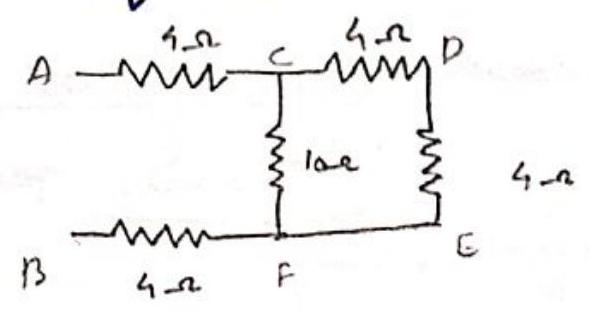
\includegraphics[max width=\figwidth]{2024_06_15_f9b8f5fbbfa74e15de4eg-1}
\end{center}

\ans

\rfloatingimg{2024_06_15_f9b8f5fbbfa74e15de4eg-1(1)}

CDE contains resistors in series

$\therefore$ CDE combines to $8 \Omega$.

\bigskip

$FG\ \&\ HA$ are in parallel.

$\therefore$ equivalent resistance $=\left(\frac{1}{10}+\frac{1}{8}\right)^{-1}=\frac{80}{18}=\frac{40}{9} \Omega$

\bigskip

Remaining resistors are in series:

$\therefore \text { equivalent resistance }=4+4+\frac{40}{9}=\frac{102}{9} = 11.3\Omega$

\usubsection{Series Connection}

When two components are in series

\begin{itemize}
	\item Current (I) flowing through them is same
	\item Have one common point \& there are no intermediate element connected to common point
	\item (may) have potential drop
\end{itemize}

\usubsection{Parallel connection}

\begin{itemize}
	\item Have same potential across the component
	\item Two ends are joined by two common points wish no element in between
\end{itemize}
\newpage
2. Find equivalent resistance across A \& B

\begin{center}
	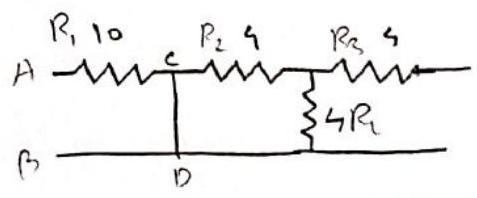
\includegraphics[max width=\figwidth]{2024_06_15_f9b8f5fbbfa74e15de4eg-2(4)}
\end{center}

\ans

$R_3$ is not fully connected. Hence it has no effect in the circuit and can be ignored.

$R_2 \& R_4$ are in series.

$\therefore$ Their effective resistance = $8 \Omega$
\bigskip

There is no resistance in $CD$ and whole current flow through $CD$ (this condition is called short circuit).

$\therefore$ net resistance is $R_1 = 10 \Omega$

\bigskip
\ques{2. Find equivalent resistance across A \& B }

\begin{center}
	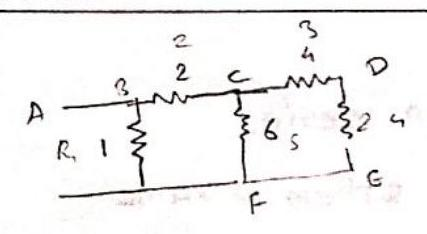
\includegraphics[max width=\figwidth]{2024_06_15_f9b8f5fbbfa74e15de4eg-2}
\end{center}

\ans

$R_3 \& R_4$ are in series, $\therefore$ their effective resistance is 6 $\Omega$

Net resistance in CDEF $=1/\left(\frac{1}{6}+\frac{1}{6}\right) = 3 \Omega = R'$

$R_E \& R'=2+3=5 \Omega = R''$

$\therefore$ Voltage across A \& B = $R_1 \| R''=\left(1+\frac{1}{5}\right)^{-1}=\frac{5}{6} \Omega$

\usubsection{Voltage Source in series}

\begin{center}
	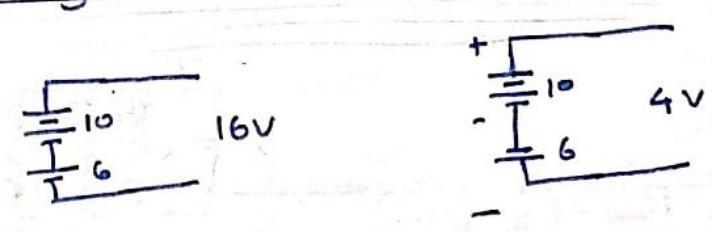
\includegraphics[max width=\figwidth]{2024_06_15_f9b8f5fbbfa74e15de4eg-2(1)}
\end{center}

\textbf{Kirchoff's voltage law}: Algebraic sum of potential drop acre a loop is zero

\rfloatingimg{2024_06_15_f9b8f5fbbfa74e15de4eg-2(2)}
$$
	\begin{aligned}
		E & =V_{1}+V_{2} \\
		  & =I R_1+I R_2
	\end{aligned}
$$

\textbf{Kirchoff's Current law}: Algebraic sum of current Howing through junction is zero
($I_{\text {in }}=I_{\text {our }}$)

\ussubsection{Voltage Divider Rule (VDR)}

\begin{center}
	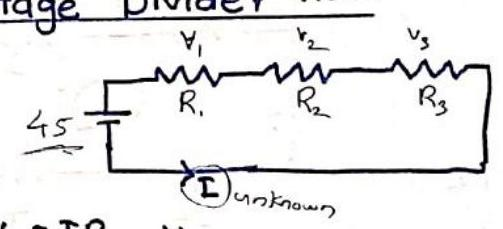
\includegraphics[max width=\figwidth]{2024_06_15_f9b8f5fbbfa74e15de4eg-2(3)}
\end{center}

$$
	\begin{aligned}
		 & R_1=2 K \\
		 & R_2=5 K \\
		 & R_3=8 K
	\end{aligned}
$$

$$
	\begin{aligned}
		 & V_n = I R_{n_0} \quad V                                                                                                                                                                  \\
		 & \text { or } V_n=\frac{R_{n} \times V}{R_T}                                                                                                                                              \\
		 & R_T = \text { total resistance }                                                                                                                                                         \\
		 & V=\text { total voltage }                                                                                                                                                                \\
		 & \therefore \underbrace{V_{1}=\frac{2 k \times 4 s}{15 k}=6 V}_{\text {less }}, V_{2}=\frac{5 k \times 45}{15 k}=15 V, \underbrace {V_{3}=\frac{8 k \times 4 s}{15 k}=24 V}_{\text{more}} \\
		 & V_1<V_{2} \because R_1<R_2 \Rightarrow V_{\text {drop }} \propto R_{\text {rm }}
	\end{aligned}
$$

*VDR is used in analysis of series circuit

\ussubsection{Current divider rule}

\begin{flalign*}
	R_{\text {net}}=\left(\frac{1}{R_1}+\frac{1}{R_2}+\ldots\right)^{-1} &  &
\end{flalign*}

$$
	\begin{rcases}
		I_{1}=I \cdot R_1^{-1} \cdot\left(\frac{R_1+R_2}{R_1 R_2}\right)^{-1}=I \cdot \frac{R_2}{R_1+R_2} \\
		I_{2}=I \cdot R_2^{-1}\left(\frac{R_1+R_2}{R_1 R_2}\right)^{-1}=I \cdot \frac{R_1}{R_1+R_2}       \\
	\end{rcases}
	\quad
	\begin{array}{r@{\;}l} % make space to RHS of \in and = symbols equal to that used for mathrel items
		\text { for } 2-\text { branch circuits }
	\end{array}
$$

\begin{flalign*}
	\boxed{I_{n}=I \cdot \frac{R_{\text {net }}}{R_{n}}} &  &
\end{flalign*}

\usubsection{Maxwell's Loup Current Method}
1. Determine current in $4 \Omega$ branch.

\rfloatingimg{mwlcm}

\ans

In loop I
\begin{flalign*}%
	\hspace*{1cm}%
	 & 1 \times\left(I_{1}-I_{2}\right)+3 \times\left(I_{1}+I_{3}\right)+4 \times I_{1}=24 &  & \\
	 & 8 I_{1}-I_{2}+3 I_{3}=24                                                            &  &
\end{flalign*}

In loop II
\begin{flalign*}
	\hspace*{1cm}
	 & 2 \cdot I_{2}+\left(I_{2}+I_{3}\right) 12+1 \times\left(I_{2}-I_{1}\right)=12 &  & \\
	 & -I_{1}+15 I_{2}+12 I_{3}=12                                                   &  &
\end{flalign*}

In loop III
\begin{flalign*}
	\hspace*{1cm}
	 & 2 I_{3}+12\left(I_{2}+I_{3}\right)+3 \cdot\left(I_{1}+I_{3}\right)=10 &  & \\
	 & 3 I_{1}+12 I_{2}+17 I_{3}=10                                          &  &
\end{flalign*}


% \begin{center}
% 	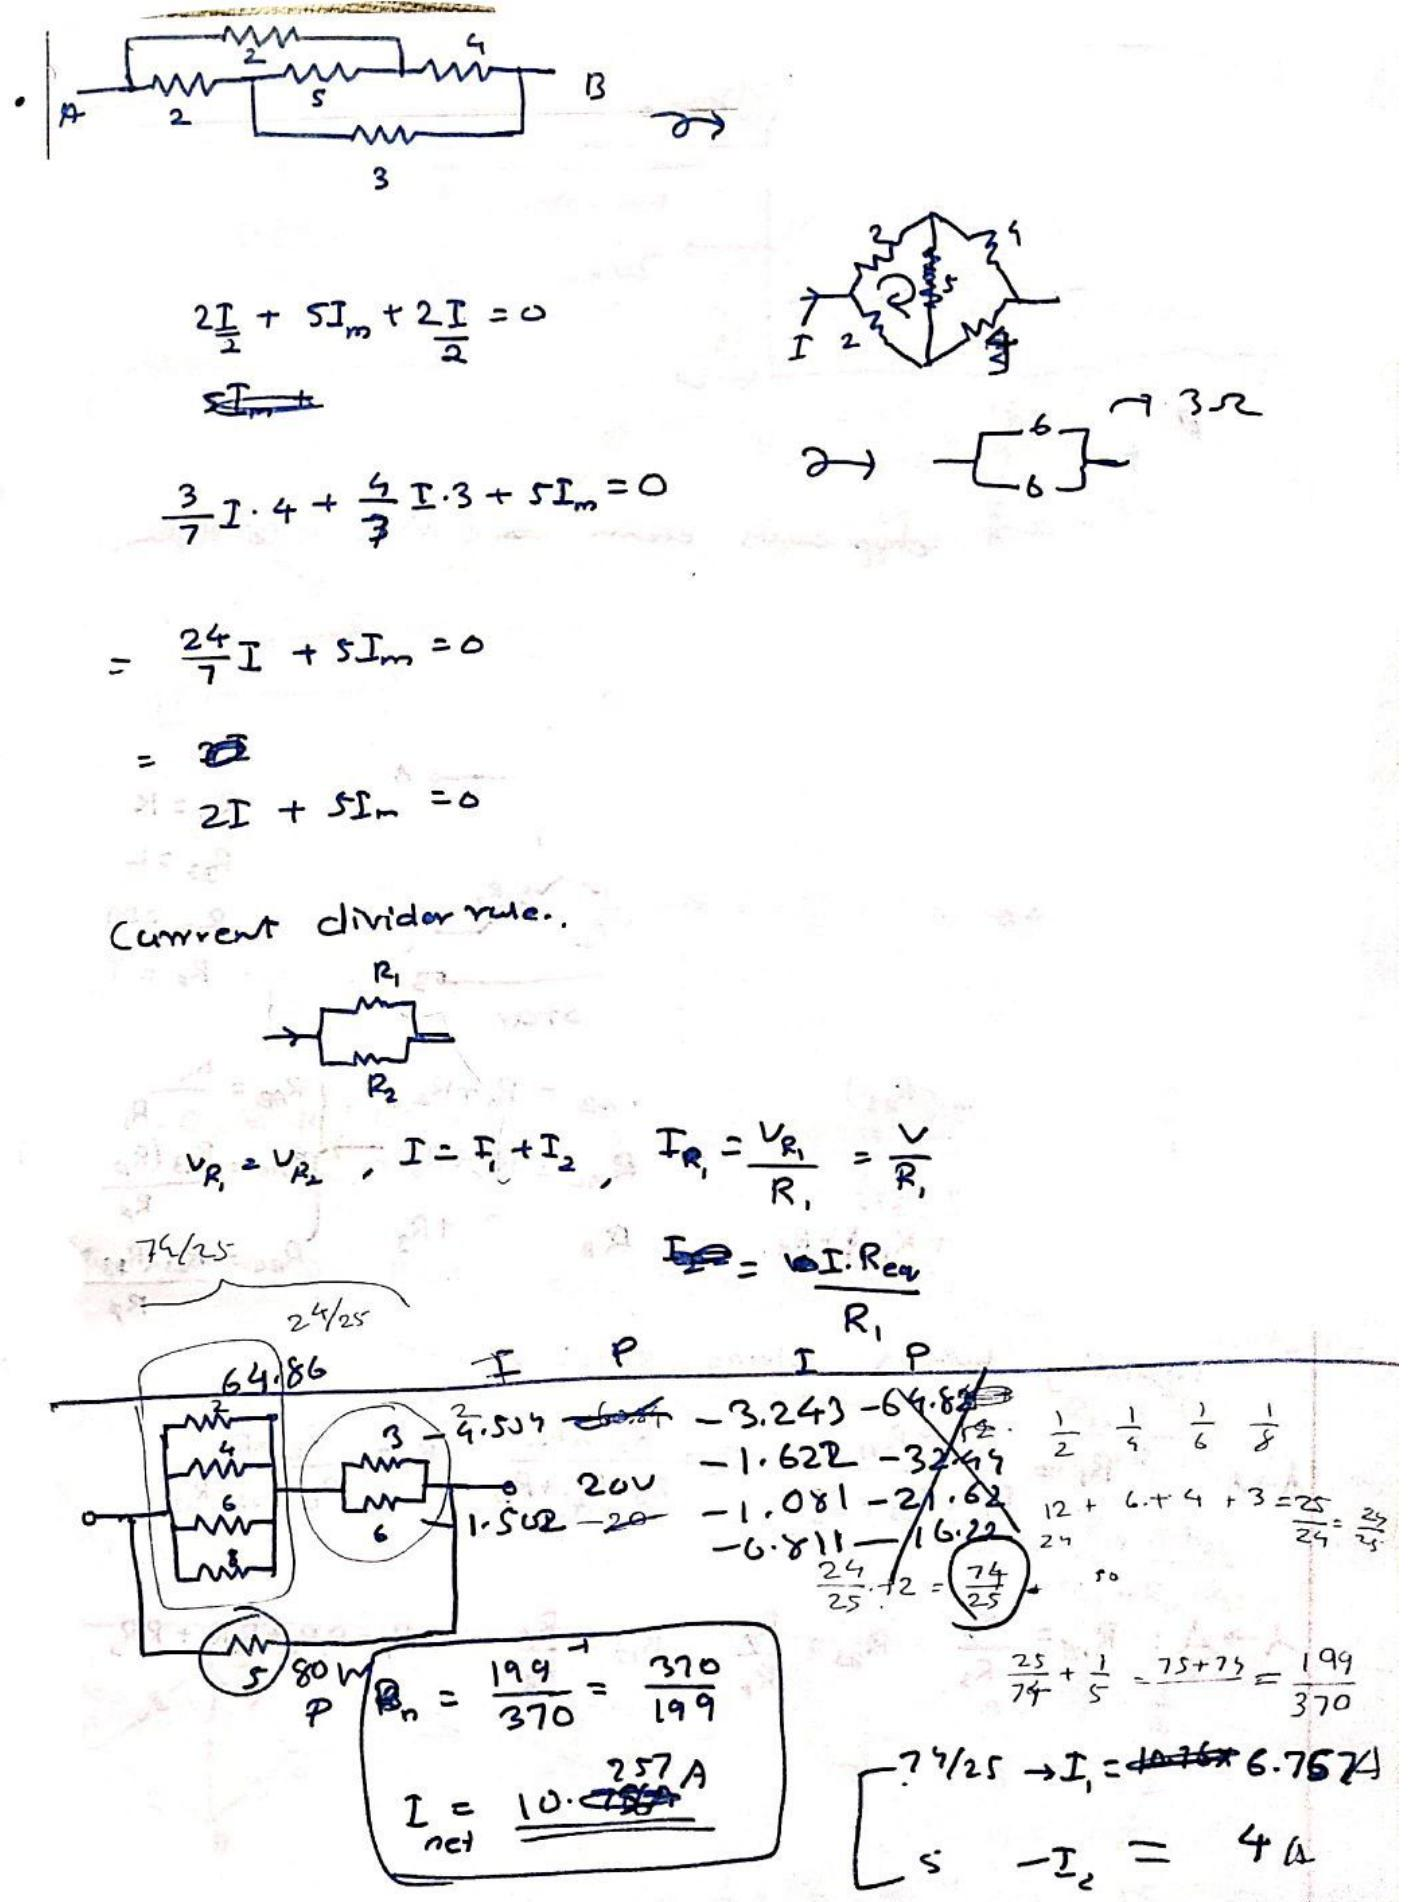
\includegraphics[max width=\figwidth]{2024_06_15_f9b8f5fbbfa74e15de4eg-3}
% \end{center}
% 
% $$
% 	\begin{aligned}
% 		 & 2 \frac{2 I}{2}+5 I_{m}+\frac{2 I}{2}=0               \\
% 		 & 5 I_{m}                                               \\
% 		 & \frac{3}{7} I \cdot 4+\frac{4}{7} I \cdot 3+5 I_{m}=0 \\
% 		 & =\frac{24}{7} I+5 I_{m}=0
% 	\end{aligned}
% $$
% 
% \begin{center}
% 	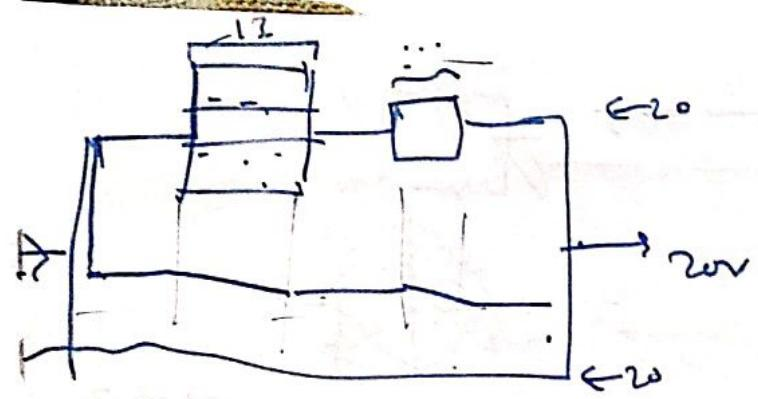
\includegraphics[max width=\figwidth]{2024_06_15_f9b8f5fbbfa74e15de4eg-4(3)}
% \end{center}

% "co-potatur chop corrss chem \& dinde wity of pom.

\usubsection{Star Deltra transformation}
\begin{figure}[h]
	\begin{subfigure}{\floatfigwidth}
		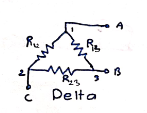
\includegraphics[width=\floatfigwidth]{delta}
	\end{subfigure}
	\begin{subfigure}{\floatfigwidth}
		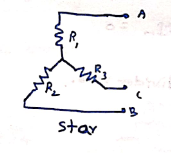
\includegraphics[width=\floatfigwidth]{star}
	\end{subfigure}
\end{figure}

\par\noindent\hspace{60pt}%
\begin{minipage}{\dimexpr\textwidth-70pt} % 60pt+10pt (left+right margin)
	\begin{flalign*}
		R_{A B} & =R_{13} \|\left(R_{12}+R_{23}\right)                           & R_{A B} & =R_{13} \|\left(R_{12}+R_{23}\right)                           & R_{A B} & =R_{13} \|\left(R_{12}+R_{23}\right)                           \\
		        & =\frac{R_{13}\left(R_{12}+R_{23}\right)}{R_{12}+R_{23}+R_{13}} &         & =\frac{R_{13}\left(R_{12}+R_{23}\right)}{R_{12}+R_{23}+R_{13}} &         & =\frac{R_{13}\left(R_{12}+R_{23}\right)}{R_{12}+R_{23}+R_{13}}
	\end{flalign*}
\end{minipage}

\begin{center}
	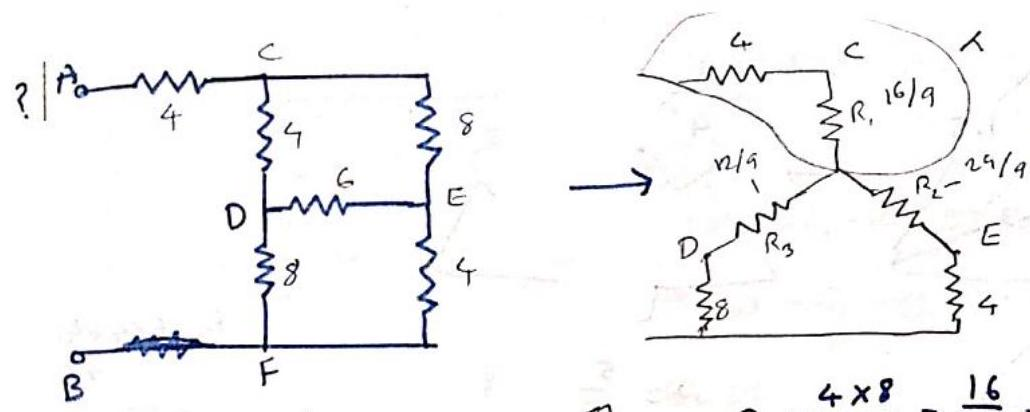
\includegraphics[max width=\figwidth]{2024_06_15_f9b8f5fbbfa74e15de4eg-4(2)}
\end{center}

$$
	\begin{aligned}
		 & R_1=\frac{4 \times 8}{4+8+6}=\frac{16}{9} \Omega                 \\
		 & R_2=\frac{6 \times 8}{18}=\frac{8}{3} \Omega=\frac{24}{9} \Omega \\
		 & R_3=\frac{6 \times 4}{18}=\frac{12}{9} \Omega \quad \frac{4}{9}
	\end{aligned}
$$

$-4-16 / 9-\left[\begin{array}{c}\frac{24}{9}-4 \\ \frac{12}{9}-8\end{array}\right]$

$$
	\begin{aligned}
		\rightarrow 4+\frac{16}{9}+\left(\frac{23}{20}+\frac{3}{28}\right)^{-1} & =4+\frac{16}{9}+\frac{560}{144} \\
		                                                                        & =47+\frac{29}{3} \Omega
	\end{aligned}
$$

$$
	\begin{aligned}
		 & R_1+R_2=\frac{K(L+m)}{T}, R_1+R_3=\frac{M(K+K)}{T}, R_2+R_3=\frac{L(K+M}{T}                                                   \\
		 & R_1=\frac{C+(2)-(3)}{2}=\frac{K L+K M+K M+M L-K L-M L}{2 T}=\frac{K M}{T}=\frac{R_{12} \times R_{13}}{R_{12}+R_{13}+R_{23}}   \\
		 & R_2=\frac{(3)-(2)+(0)}{2}=\frac{K L+M L-K M-M L+K M+K L}{2 T}=\frac{K L}{T}=\frac{R_{12} \times R_{23}}{R_{12}+R_{13}+R_{23}} \\
		 & R_3=\frac{(2)-(1)}{2}=\frac{K M+M L-K L-K M+K L+M L}{2 T}=\frac{M L}{T}=\frac{R_{13} \times R_{23}}{R_{12}+R_{13}+R_{23}}
	\end{aligned}
$$

\begin{center}
	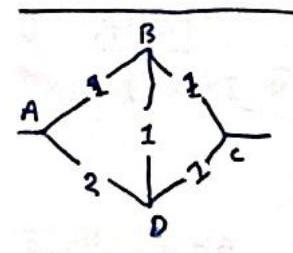
\includegraphics[max width=\figwidth]{2024_06_15_f9b8f5fbbfa74e15de4eg-4}
\end{center}

$$
	\begin{aligned}
		 & \rightarrow \underbrace{1 / 2}_{2} \rightarrow \underbrace{1 / 2}_{1 / 2}                                               \\
		 & A=\frac{1 \times 2}{4}=\frac{1}{2}                                                                                      \\
		 & B=\frac{1}{2}                                                                                                           \\
		 & c=\frac{1}{4}                                                                                                           \\
		 & \rightarrow \frac{1}{2}+\left(\frac{2}{3}+\frac{5}{5}\right)^{-1}=\frac{1}{2}+\frac{15}{22}=\frac{52}{44}=\frac{26}{22} \\
		 & =\frac{13}{11}-3
	\end{aligned}
$$

$$
	1 \rightarrow \rightarrow: R_{12}=\frac{R_{\varphi}}{R_3} \quad R_{23}=\frac{R_{\psi}}{R_{p}} \quad R_{13}=\frac{R_{\psi}}{R_2} \quad R_4=R_1 R_2+R_2 R_3+R_1 R_3
$$

\begin{center}
	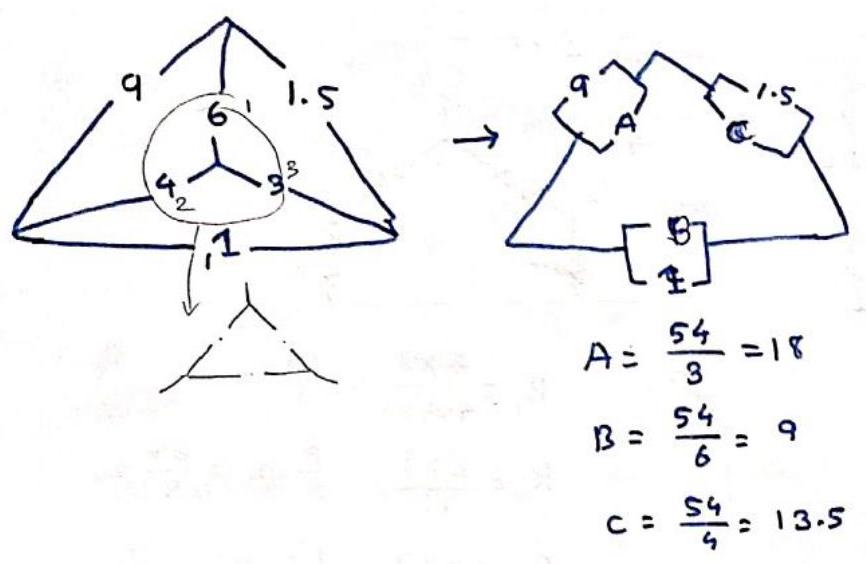
\includegraphics[max width=\figwidth]{2024_06_15_f9b8f5fbbfa74e15de4eg-5(3)}
\end{center}

1.

\begin{center}
	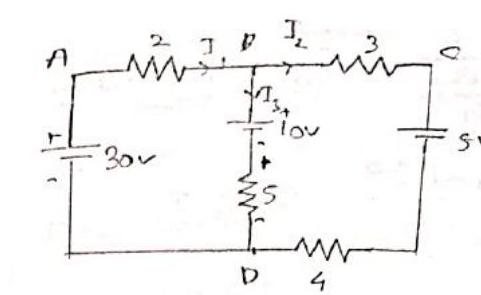
\includegraphics[max width=\figwidth]{2024_06_15_f9b8f5fbbfa74e15de4eg-5(1)}
\end{center}

$R_{y}=6 \times 4+4 \times 3+$

$=24+12+18$ : 54 $\therefore$ reducabled: $\left(\frac{1}{9}+\frac{1}{18}\right)^{-1}=6,\left(\frac{1}{1.5}+\frac{1}{9}\right)^{-1}=\frac{9}{7}$. $\frac{1}{1}+\frac{1}{13.5}=\frac{27}{29}$\\
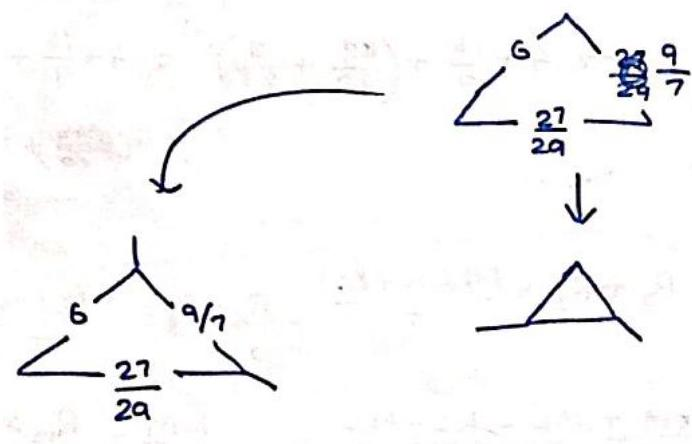
\includegraphics[max width=\textwidth, center]{2024_06_15_f9b8f5fbbfa74e15de4eg-5}

$=\frac{603}{556}$

$\frac{458}{556}$

$$
	=\frac{225}{139}
$$

mesh $\rightarrow \square$

\section*{Cromeristule}
$$
	\begin{aligned}
		\therefore I_{1} & =\frac{\Delta_{1}}{\Delta}=\frac{265}{59} \\
		I_{2}            & =\frac{\Delta_{2}}{\Delta}=\frac{135}{59}
	\end{aligned}
$$

By $\mathrm{KCL}: I_{3}=I_{1}-I_{2}$

ABDA:

$+30-2 I_{1}-10-5 I_{3}=0$

$\Rightarrow$ 20 $-7 I_{1}+5 I_{2}+20=0 \Rightarrow 7 I_{1}-5 I_{2}=20$

\section*{$B C D B$}
$-3 I_{2}-5-4 I_{2}+8 I_{3}+10=0$

$\Rightarrow 5 I_{1}-12 I_{2}=-5$

$$
	\therefore \quad I_{1}=\frac{265}{59}, \quad I_{2}=\frac{135}{59}
$$

$$
	\begin{aligned}
		 & {\left[\begin{array}{cc}
						          7 & -5  \\
						          5 & -12
					          \end{array}\right]\left[\begin{array}{l}
						                                  I_{1} \\
						                                  T_{2}
					                                  \end{array}\right]=\left[\begin{array}{l}
						                                                           20 \\
						                                                           C_{1}
					                                                           \end{array}\right]} \\
		 & \Delta=\left|\begin{array}{ll}
			                7 & -5  \\
			                5 & -12
		                \end{array}\right|=-59                                         \\
		 & \begin{array}{l}
			   \text { Replar } C_{n} \text { by } R \\
			   n^{m} U v=\frac{U_{n}}{\Delta}
		   \end{array}
	\end{aligned}
$$

$$
	\begin{aligned}
		 & \Delta_{1}=\left|\begin{array}{cc}
			                    20 & -5  \\
			                    -5 & -12
		                    \end{array}\right|=-265 \\
		 & \Delta_{2}=\left|\begin{array}{cc}
			                    7 & 20 \\
			                    5 & -5
		                    \end{array}\right|=-135
	\end{aligned}
$$

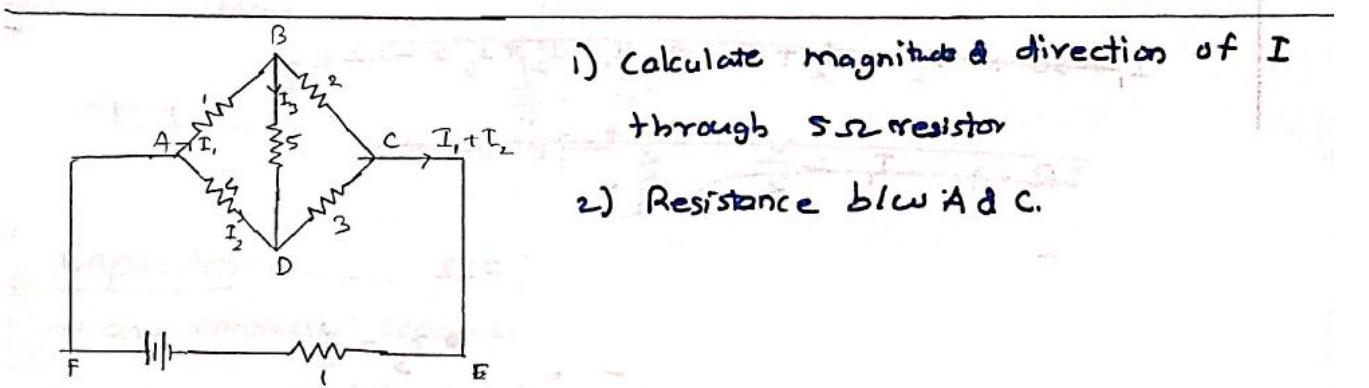
\includegraphics[max width=\textwidth, center]{2024_06_15_f9b8f5fbbfa74e15de4eg-5(2)}\\
a) $\quad \triangle B D A: \quad$ b) $B C D B$

$$
	I_{1}+5 I_{3}-4 I_{2}=0-\omega \quad 2\left(I_{1}-I_{3}\right)-3\left(I_{2}+I_{3}\right)-5 I_{3}=0
$$

$$
	\Rightarrow 2 I,-3 I_{2}-10 I_{3}=0
$$

\begin{enumerate}
	\setcounter{enumi}{7}
	\item $A B C E F A$
\end{enumerate}

$$
	\begin{aligned}
		 & I_{1}+2\left(T_{1}-I_{3}\right)+I_{1}+I_{2}-4=0 \\
		 & 4 I_{1}-I_{2}-2 I_{3}-4=0
	\end{aligned}
$$

$\Rightarrow I_{1}=\frac{31}{28} \quad I_{2}=-\frac{1}{28}-0.34$

$I_{3}=\frac{13}{56} \approx 0.232 \mathrm{~A}-0.087$ $\therefore$ 1) from $B \rightarrow D$

$$
	\begin{aligned}
		 & \text { 2) } R_{\text {net }}=\frac{V}{I}=                                \\
		 & \frac{4}{\frac{15}{14}+1}=\frac{56}{29} \approx 1.931 . \mathrm{A} \Omega
	\end{aligned}
$$

\begin{center}
	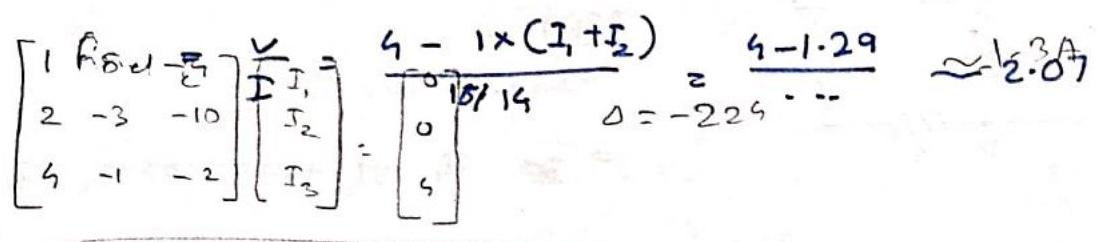
\includegraphics[max width=\figwidth]{2024_06_15_f9b8f5fbbfa74e15de4eg-6(4)}
\end{center}

$$
	\begin{aligned}
		 & \left.\left[\begin{array}{ccc}
				               1 & 5  & 0 \\
				               2 & -3 & 0 \\
				               4 & -1 & 4
			               \end{array}\right] \quad \Delta_{3}=-52\right]\left|\begin{array}{ccc}
			                                                                   0 & 5  & -4  \\
			                                                                   0 & -3 & -10 \\
			                                                                   4 & -1 & -2
		                                                                   \end{array}\right| \quad \Delta_{1}= \pm 248
	\end{aligned}
$$

$$
	\left|\begin{array}{lll}
		1 & 0 & -4  \\
		2 & 0 & -10 \\
		4 & 4 & -2
	\end{array}\right| \quad 0_{2}=8
$$

$$
	\begin{aligned}
		 & I_{1}=\frac{\Delta_{1}}{\Delta_{4}}=+\frac{31}{28}, \quad I_{2}=-\frac{1}{28} \\
		 & I_{3}=\frac{13}{56}
	\end{aligned}
$$

\begin{center}
	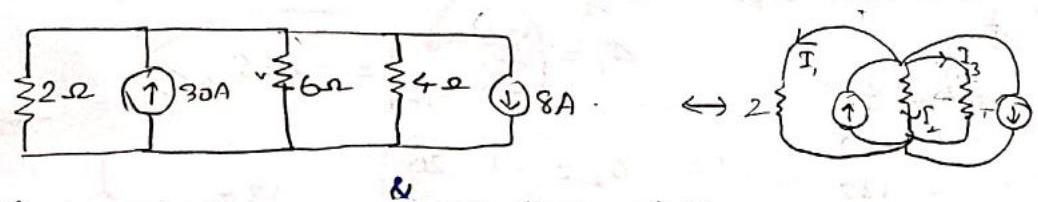
\includegraphics[max width=\figwidth]{2024_06_15_f9b8f5fbbfa74e15de4eg-6(2)}
\end{center}

\begin{enumerate}
	\item Find polarity $\&$ magnitude of $v$
\end{enumerate}

$$
	\begin{aligned}
		 & I_{1}+I_{2}+I_{3}+8=030 \Rightarrow I_{1}+\frac{V}{2}+I_{3}=22 \\
		 & I_{2}=\frac{V}{6}, \quad I_{3}=\frac{V}{4}                     \\
		 & \frac{V}{2}+\frac{U}{6}+\frac{U}{4}=22                         \\
		 & 24 V+8 V+12 V=22 \times 48                                     \\
		 & \Rightarrow \quad U=24 V
	\end{aligned}
$$

IDeal voltage source

$\rightarrow$ zero internal vereristance

$\rightarrow$ Supply constr. voltage at all currents

Real voltage source

\begin{center}
	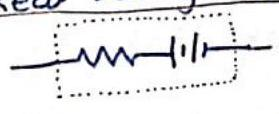
\includegraphics[max width=\figwidth]{2024_06_15_f9b8f5fbbfa74e15de4eg-6}
\end{center}

\begin{itemize}
	\item voltage source with very low internal resistance. can be treated as constant voltage source
\end{itemize}

Ideal Current source $(-\Theta-)$

Real current Source.

$\rightarrow \infty$ internal resistance winy? M $\Theta$

$\rightarrow$ supply constr. Current at all loads

Source conversion

\begin{center}
	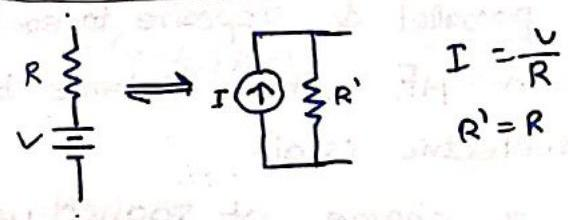
\includegraphics[max width=\figwidth]{2024_06_15_f9b8f5fbbfa74e15de4eg-6(3)}
\end{center}

\begin{center}
	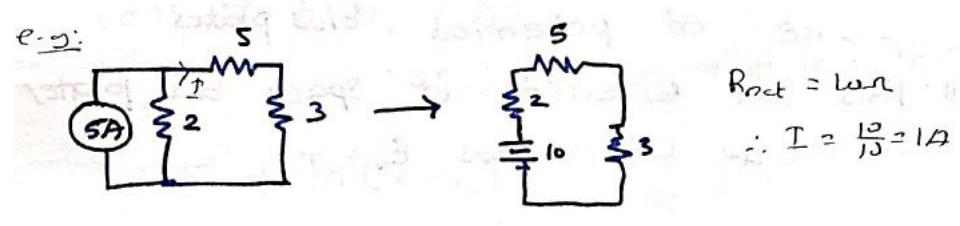
\includegraphics[max width=\figwidth]{2024_06_15_f9b8f5fbbfa74e15de4eg-6(5)}
\end{center}

Capacitor

〜 any conductor separated by insulator (alielectsc)

Capacitance: Ability of capacitorto store energy. (change $\rightarrow$ Ublwiwn) Dielectrics: air, mica, waxedpaper, ceramic, electrolyte

\begin{center}
	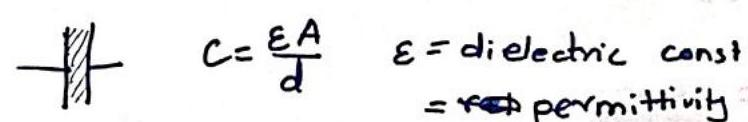
\includegraphics[max width=\figwidth]{2024_06_15_f9b8f5fbbfa74e15de4eg-6(1)}
\end{center}

$$
	=\text { permittivity }=\varepsilon_{0} \cdot \varepsilon_{r} \text {. }
$$

Energy stored: $\frac{1}{2} C v^{2}=\frac{1}{2} Q v=\frac{1}{2} Q^{2} / C$

\begin{center}
	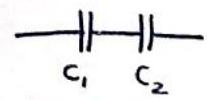
\includegraphics[max width=\figwidth]{2024_06_15_f9b8f5fbbfa74e15de4eg-7}
\end{center}

$$
	\begin{aligned}
		 & c=\left(\frac{1}{c_{1}}+\frac{1}{c_{2}}\right)^{-1}             \\
		 & v_{1}=\operatorname{pd}\left(c_{1}\right)                       \\
		 & v_{2}=\operatorname{pdd}\left(c_{2}\right)                      \\
		 & Q_{1}=Q_{2}=Q                                                   \\
		 & \therefore V=v_{1}+v_{2}                                        \\
		 & \frac{Q}{C}=\frac{Q_{1}}{c_{1}}+\frac{Q}{c_{2}}                 \\
		 & \Rightarrow C=\left(\frac{1}{c_{1}}+\frac{1}{c_{2}}\right)^{-1}
	\end{aligned}
$$

\begin{enumerate}
	\item A capacitor consists of two similar square Al. plates each $10 \mathrm{~cm} \times 10 \mathrm{~cm}$ bounded parallel \& opposite to each other. what is their capacitance in MF when distance blu them is $1 \mathrm{~cm} \&$ deedielectric is air
\end{enumerate}

ii) If capacitor is given a charge of soomfic what will be difference of potential blur plates

iii) How will this be effected if space bow plates is filled with wax which has $\varepsilon_{r}=4$

A.

$$
	\begin{aligned}
		c=\frac{\varepsilon_{0} \varepsilon_{r} A}{d}=\frac{\varepsilon_{0} \times \varepsilon_{4}^{1} \times(10 \times 10) \times 10^{-4}}{10^{2}} & =8.85 \times 10^{-12} \mathrm{~F}   \\
		                                                                                                                                            & =8.85 \times 10^{-1} \mu \mathrm{F}
	\end{aligned}
$$

iii) $V=\frac{Q}{c}=\frac{500 \mu \mathrm{K}_{4} c}{8.85 \times 10^{-1} / \mu F}=56.47 \mathrm{~V}$

iii) $v=\frac{Q}{C^{\prime}}=\frac{C Q}{4 C}=19.12 V$
At $t=R C$ :

$$
	\begin{aligned}
		v_{c} & =v\left(1-e^{-R c / R_{c}}\right) \\
		      & =0.632 . v
	\end{aligned}
$$

$$
	\begin{aligned}
		I_{0} & =I_{m} \cdot e^{-R c / R c} \\
		      & =0.368 I_{m}
	\end{aligned}
$$

RC : time cunstant:: Time at which the voltage across $G(\tau, \lambda)$ the capacitor reaches $63.2 \%$ of steady state $T$. voltage / current reaches $36.8 \%$ of initial value.

If $t=2 R C$ :

$$
	\begin{aligned}
		 & v_{c}=v\left(1-e^{-2}\right)=0.865 . \mathrm{V} \\
		 & t=S R C, v_{c}=0.993 \mathrm{~V}
	\end{aligned}
$$

Rate of Rise of voltage.

$$
	v=R C \cdot \frac{d v_{c}}{d t}+v_{c}
$$

at $t=0, v_{c}=0$

$$
	\begin{aligned}
		 & =0, v_{c}=0                                                                                                                      \\
		 & \therefore v=R C \cdot \frac{d v_{c}}{d t} \Rightarrow \frac{d v_{c}}{d t}=\frac{v}{R c} \quad \begin{array}{l}
			                                                                                                  \text { initicl rate of-rise in } \\
			                                                                                                  \text { voltage (acrosy capacion }
		                                                                                                  \end{array}
	\end{aligned}
$$

1.

A $2 \mu \mathrm{f}$ capacitor is connected by closing a switch to a supply of $100 \mathrm{~V}$ through a $1 \mathrm{M} \Omega$ series resistance. Calculate.

i) Time constant ii) Initial charging current iii) $\left.\frac{d v_{c}}{d t}\right|_{t=0}$ iv) Voltaye across capacitor \&s after the switch has been closed

v) Time token for capacitor to be fully charged

ii) $I_{m}=\frac{V}{R}=\frac{100}{10^{6}}=10^{-4} \mathrm{~A}=109 \mathrm{~A}$ iii) $\left.\quad \frac{d v_{c}}{d t}\right|_{f=0}=\frac{v}{R c}=\frac{100}{2}=50 \mathrm{~V} / \mathrm{s}$

iv) $v_{c}=v\left(1-e^{-t / \tau}\right)$

$$
	=100\left(1-e^{-6 / 2}\right)=95.02 \mathrm{~V}
$$

v) $\infty$ Q? I $a=c v \Rightarrow c v\left(1-e^{-t / \tau}\right)=c \cdot v$ (to fully charge)

$$
	\begin{aligned}
		\Rightarrow 1-e^{-t / \tau} & =1                      \\
		-e^{-t / \tau}              & =0 \Rightarrow t=\infty
	\end{aligned}
$$

llor take $5 \mathrm{~T}=105$

Discharging of Capacitor

At $t=0: V_{c}=V$

$$
	I=0
$$

\begin{center}
	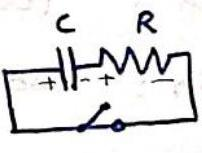
\includegraphics[max width=\figwidth]{2024_06_15_ae1c13e212c06c234cc4g-01(1)}
\end{center}

$t>0$ :

$$
	\begin{aligned}
		 & \text { Applying KvL: }                                                                                                                         \\
		 & \qquad \begin{aligned}
			          v_{c}+I R=0 \Rightarrow & v_{c}+R c \cdot \frac{d v_{c}}{d t}=0                        \\
			                                  & \Rightarrow \frac{d v_{c}}{v_{c}}=-\frac{d t}{R c}           \\
			                                  & \Rightarrow \int \frac{d v_{c}}{v_{c}}=-\int \frac{d t}{R c} \\
			                                  & =\ln \left(v_{c}\right)=-t / R c+k
		          \end{aligned}
	\end{aligned}
$$

to find $k, t=0, v_{c}=v$

$$
	\ln \left(x_{0}\right)=k
$$

$$
	\therefore(1) \equiv \ln \left(v_{c}\right)=-t / R C+\ln (v)
$$

\begin{center}
	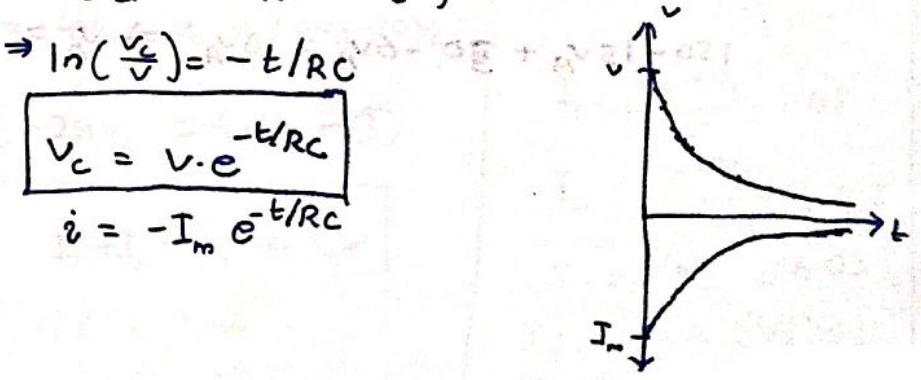
\includegraphics[max width=\figwidth]{2024_06_15_ae1c13e212c06c234cc4g-01.jpg}
\end{center}

2. A cable lo km long and of capacitance $2.5 \mu \mathrm{F}$ discharges through its insulation resistance of $50 \mathrm{M} \Omega$ By what percentage the corvoltage would have fallen 1,2, \& 5 mons. respectively. After disconnection from bus-bars
A) $V_c=V\left(1-e^{-L / \tau}\right) \quad T=R C=50 \times 10^6 \times 10^{-6} \times 2.5=1255$
at 1min: $\frac{v_{-}-v_2}{v^{10100}}=100\left(1-e^{-60 / 125}\right)=37.12 \%$
at $2 \mathrm{~min}: 100\left(1-e^{-120 / 125}\right)=61.71 \%$
at $5 \mathrm{~min}$ : $100\left(1-e^{-300 / 125}\right)=90.93 \%$
Nodal Analysis
Potential at $A$ :
By $K \subset L: I_3=I_1+I_2$
$$
	\begin{aligned}
		I_1=       & \frac{V_{2 A} 0}{2}=\frac{V_B-V_A}{2 Q}=\frac{10-V_A}{2}                        \\
		I_2=       & \frac{5-V_A}{5}, I_3=\frac{V_A-0}{3}                                            \\
		\therefore & 5-\frac{V_A}{2}+1-\frac{V_A}{5}=\frac{V_A}{3}                                   \\
		           & 150-15 V_A+30-6 V_A=10 V_A \Rightarrow V_A=\frac{-280}{31}=2 \frac{180}{31} . V
	\end{aligned}
$$
ut A:
$$
	\begin{aligned}
		 & 10=I_1+I_2+I_3                                       \\
		 & 10=\frac{V_A-V_C}{5}+\frac{V_A-V_B}{3}+\frac{V_A}{2} \\
		 & 300=6 V_A-6 V_C+10 V_A-10 V_B+15 V_A
	\end{aligned}
$$
$10 A$
$$
	31 v_A-10 v_B-6 v_C=300
$$

At B:
$$
	\begin{aligned}
		 & I_2+I_4+I_5=0                                           \\
		 & \frac{V_A-V_B}{3} \pm \frac{V_B}{5}+\frac{V_B-V_C}{1}=0 \\
		 & 5 V_A-5 V_B \pm 3 V_B+15 V_B-15 V_C=0                   \\
		 & -5 V_A+83 V_B+15 V_C=0 \text {-(2) }
	\end{aligned}
$$

At c:
$$
	2+I_6=I_1+I_5
$$
$$
	\begin{aligned}
		 & \text { (2. } 1 \\
		 & 5 .-1           \\
		 & 3.8
	\end{aligned}
$$
$$
	2+\frac{v_C}{4}=\frac{v_A-v_C}{5}+\frac{v_B-v_C}{1}
$$
$$
	\begin{aligned}
		 & \Rightarrow 40+5 v_c=4 v_A-4 v_C+20 v_B-20 v_c \\
		 & \Rightarrow 4 v_A+20 v_B-29 v_C=40
	\end{aligned}
$$
(also true, but $\infty$ into. About ign $)$

\begin{center}
	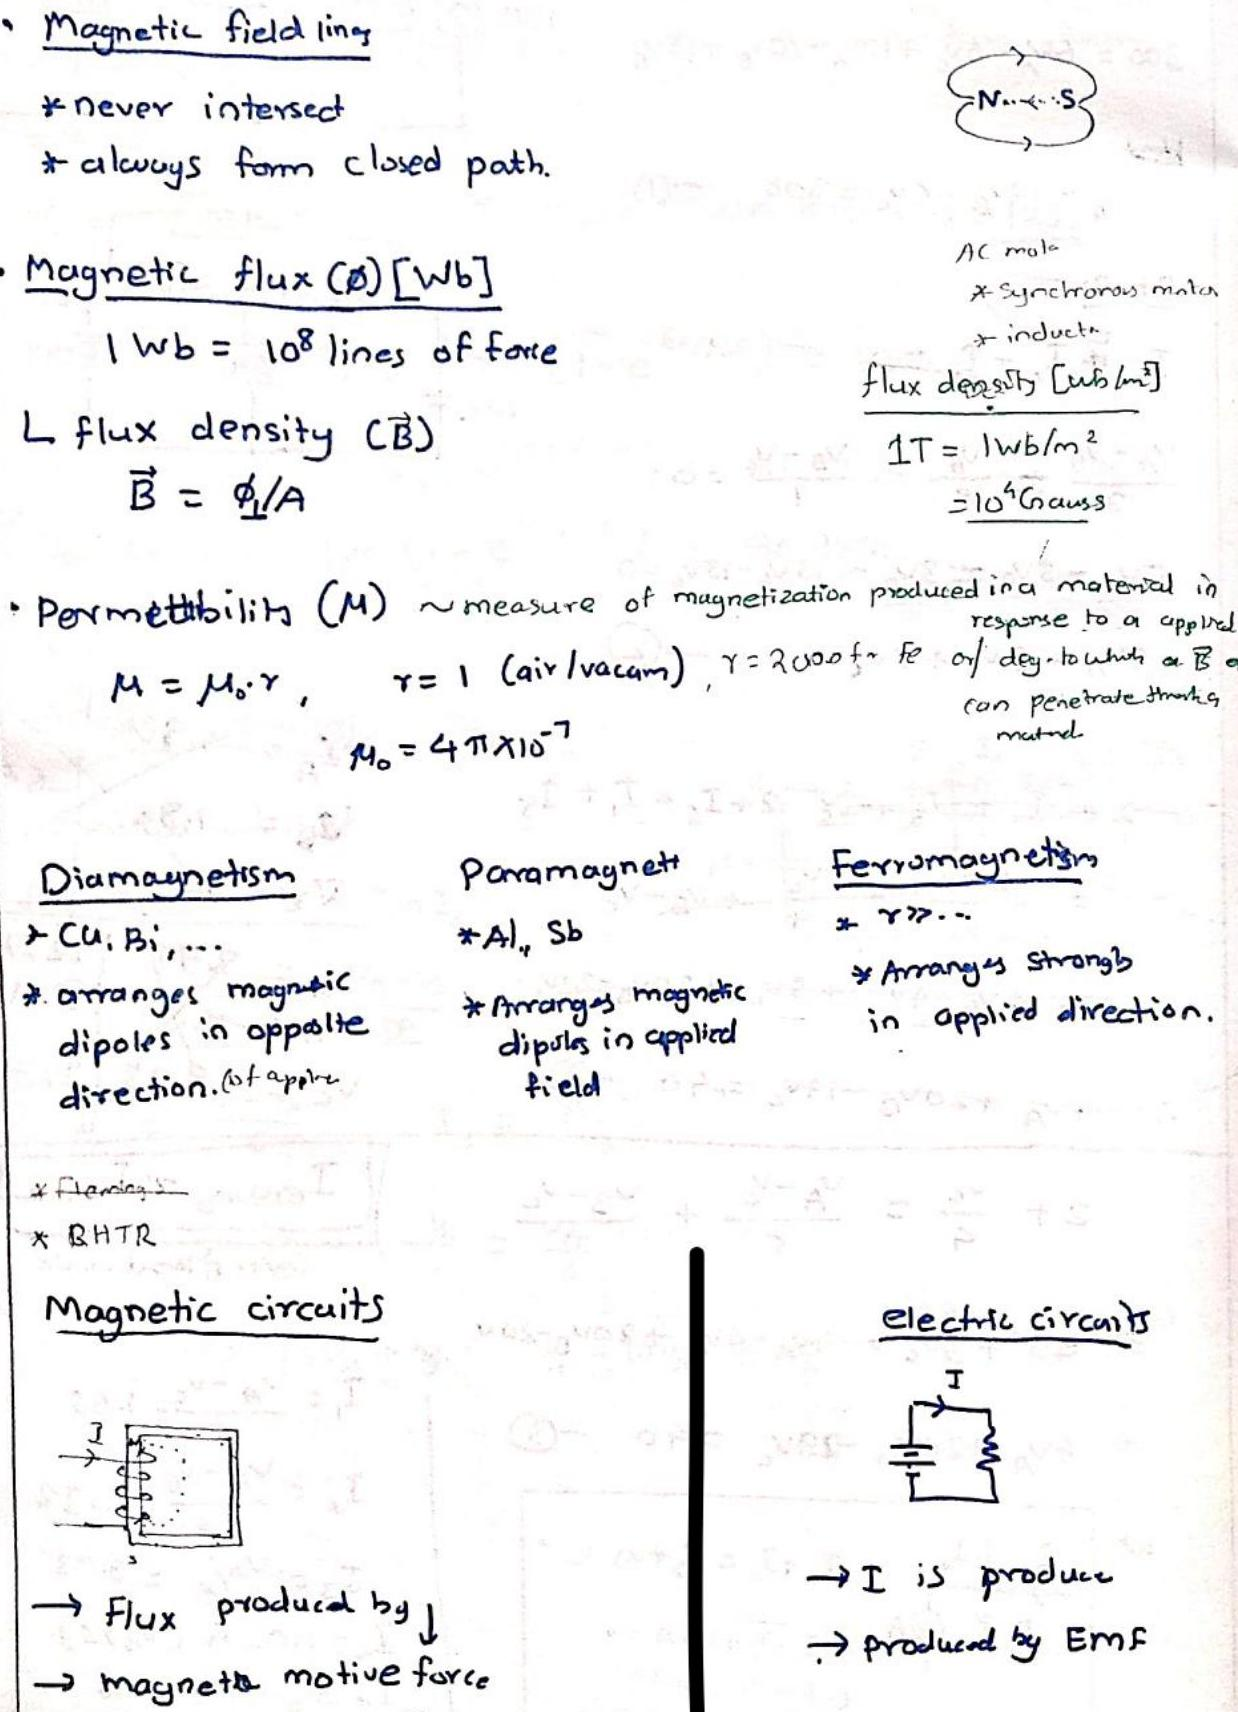
\includegraphics[max width=\figwidth]{2024_06_15_ae1c13e212c06c234cc4g-03.jpg}
\end{center}

Here, there's resistarlo:

$$
	R=p_{2}
$$

$\sim$ Reluctance

$$
	\text { eryg's of anducto }
$$

$$
	S=\frac{2}{\mu a} \text { y aroa of erross section of ming circuit }
$$

$\rightarrow \phi=\frac{m m f}{s}=\frac{N I}{s 1} \cdot \mu \cdot a \cdot \mu$.

$=\frac{M \cdot N I_{a}}{2}$

$\rightarrow$ Tows deroun $n$ ? matenat:

$\rightarrow$ No drop in fower

due to flum

$\rightarrow$ Permeance

$\rightarrow$ Permeabilly

$\rightarrow$ doesn't flow actually

$\rightarrow$ No magnetrc insulator ?

$\rightarrow$ Permeability depends on the max. flux density $\left(B_{\text {mea }}\right)$ and it isn't constam

\begin{itemize}
	\item Magnetir field interslts (H)
\end{itemize}

$$
	H=\frac{B}{\mu}=\frac{N I}{2}
$$

men $\phi=\frac{\mu \cdot \Lambda I_{a}}{2} \Rightarrow B=\frac{\mu N I}{2}$

or $1 t=\frac{\omega f}{y}$

$\therefore m m t=H^{*} 2$ $\rightarrow$ opposition to I

$\rightarrow \quad I=\frac{V}{R}$

$\rightarrow$ flocors strerish the

conductors

$\rightarrow$ Poterea drop is

presen. uto res siake.

$\rightarrow$ conductance.

$\rightarrow$ conductivity

$\rightarrow$ Poes flow

$\rightarrow$ electric insulators.

$\rightarrow$ Resistivits of a material is almost constawt etcept for slight change due to change in temp.

\begin{enumerate}
	\item An Iron ring of circular cross sectional area: of $3 \mathrm{~cm}^{2}$ and mean diameter of $20 \mathrm{~cm}$ is wound with a 500 tums of wire and carries a curves of 2.09 A. to produce the magnetic flux of o.smuls in the ring. Determine the pormabills of the matoriod
\end{enumerate}

A) Given:

$$
	\begin{aligned}
		 & a=3 \mathrm{~cm}^{3} \equiv 3 \times 10^{-9} \mathrm{~m}^{2} \\
		 & d=20 \mathrm{~cm}, N=500                                     \\
		 & I=2.09 \mathrm{~A}, \phi=0.5 \times 10^{-3} \mathrm{wb}
	\end{aligned}
$$

reluctance $s=\frac{2}{\mu a}$

$$
	\begin{aligned}
		Z=\text { mean length } & =\pi \cdot d            \\
		                        & =0.2 \pi \mathrm{m}^{*}
	\end{aligned}
$$

\begin{center}
	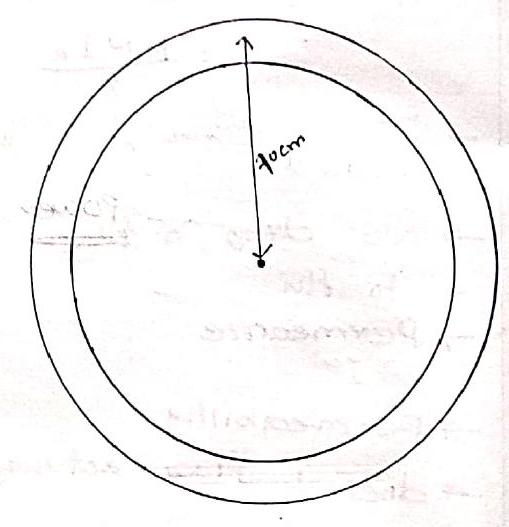
\includegraphics[max width=\figwidth]{2024_06_15_ae1c13e212c06c234cc4g-04}
\end{center}

$$
	\begin{aligned}
		 & \therefore s=\frac{l}{\mu \cdot a}                                                             \\
		 & \begin{aligned}
			   \phi=\frac{m m f}{s}=\frac{N I}{s}= & \Rightarrow 0.5 \times 10^{-3}=\frac{500 \times 2.09}{s} \\
			   \Rightarrow s=                      & 500 \times 2.09 \times 2 \times 10^{3}                   \\
			                                       & =2090000
		   \end{aligned}
	\end{aligned}
$$

$$
	\begin{aligned}
		\therefore \mu & =\frac{l}{s \cdot a}=\frac{0.2 \pi}{2090000 \times 63 \times 10^{-4}}=0.0010021 \\
		\mu_{r}        & =\frac{\mu}{4 \pi \times 10^{-7}}=797
	\end{aligned}
$$

Linear circus: liner rel. bu vuraye \& Current output ( $V \& I$ ) ane lina function of input ( $V Q I), \sim n,-A$

non-liner: rel bu Vax. is a non-liner function didos, transistors, transform whose core is sutuch

Unilateral: allows flow sf current in one direction only bilateral: ares cunt in both direction

Active elem: require eternal power to operate produce enarys, semiconductor,

\begin{itemize}
	\item passive element: doresnt generate but dissappats, stores/releors it. $R, c, I$
\end{itemize}

Series magnetic circuits

\begin{center}
	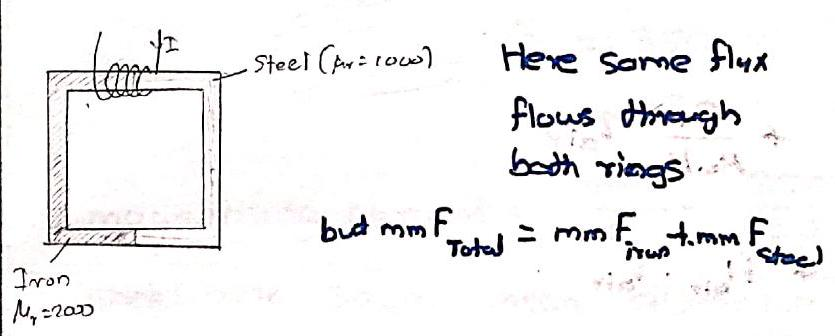
\includegraphics[max width=\figwidth]{2024_06_15_ae1c13e212c06c234cc4g-04(1)}
\end{center}

$$
	\text { but } m m F_{\text {Total }}=m m F_{\text {item }}+. m m F_{\text {steel }}
$$

Just like ina series $e^{\text {c circuits. }}$ $v=v_{1}+v_{2}$

Parallel circuits\\
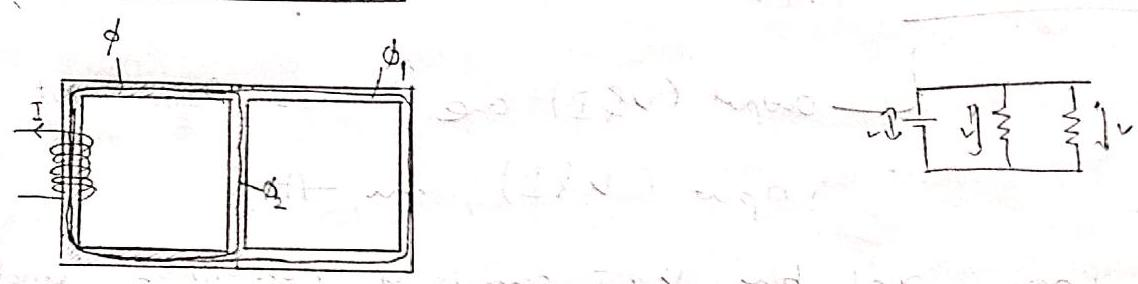
\includegraphics[max width=\textwidth, center]{2024_06_15_ae1c13e212c06c234cc4g-05}

$$
	\begin{aligned}
		m m f_{T} & =m m f_{\phi}+m m F_{\phi}     \\
		          & =m m f_{\phi}+m m f_{\phi_{2}}
	\end{aligned}
$$

$$
	\begin{aligned}
		 & m m f_{\phi_{1}}=m m f_{\phi_{2}} \\
		 & \phi=\phi_{1}+\phi_{2}
	\end{aligned}
$$

$$
	\begin{aligned}
		m m F_{T}                   & =m m f_{a i v}+m m f_{i \text { ron }}=\underset{\text { reductome }}{\phi}                                                         \\
		                            & =\phi \cdot s_{\text {iron }}+\phi \cdot s_{\text {air }} \quad s=\frac{2}{\mu a}                                                   \\
		                            & =\frac{\phi}{\mu_{0} a}\left(\frac{\tau_{\text {iron }}}{\mu_{\text {iron }}}+\frac{\tau_{\text {air }}}{\mu_{\text {air }}}\right) \\
		                            & =\frac{B}{\mu_{0}}(\cdots)                                                                                                          \\
		                            & =\frac{B}{\mu_{0}} \cdot \tau_{\text {ron }}+\frac{B .}{\mu_{0} \cdot \mu_{a i v}} \tau_{\text {air }}                              \\
		(A \cdot \text { tummy mm } & =H_{\text {iron }} \cdot \tau_{\text {iron }}+H_{\text {air }} \cdot \tau_{\text {air }}
	\end{aligned}
$$

leakage flux: flow not flowing through desired

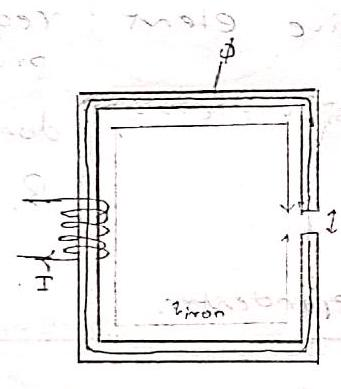
\includegraphics[max width=\textwidth, center]{2024_06_15_ae1c13e212c06c234cc4g-05(1)}\\
magnetic path

Useful flux: oflut through air gap/airflut.

\begin{itemize}
	\item leakage factor $(\lambda)=\frac{\mu \text { setal }}{\text { total }}$ Hus
	\item Fringing: Bulging of flux cot air gap
\end{itemize}

I111). A cast steel a electromagnet a hos an air gap length of $3 \mathrm{~mm}$ and an iron path length of $40 \mathrm{~cm}$. find number of ampere turns necessary to produce a flux density of $0.7 \mathrm{~Wb} / \mathrm{m}^{2}$ in the gap. neglect leakage A \& fringing. Assume A-T for airgap to be $70 \%$ of tome $A I$\\
A) $A T_{\text {air }}=\phi \cdot S_{\text {air }}=\phi \cdot \frac{2}{\mu_{0} \cdot \mu_{r} a}=B \frac{2}{\mu}=\frac{0.7 \times 3 \times 10^{-3}}{4 \times 3.14 \times 10^{-7}}=1072 A$.

$$
	\text { A.T } T_{\text {total }}=\frac{10}{7} \times 1672=2388 \text { ATT }
$$

$\phi$ - same here

\begin{itemize}
	\item An iron ring of crosse sectional area $6 \mathrm{~cm}^{2}$ is wound with a wire of 100 turns. and has a saw-cut of $2 \mathrm{~mm}$, calculate the magnetising current required to produce a flux of $0.1 \mathrm{~mW}$ if mean length of magnetic path is $30 \mathrm{~cm}$. ard $\mu_{0, \text { non }} \mu_{0} .470$\\
	      A)
\end{itemize}

$$
	\begin{aligned}
		m m f=\phi \cdot S_{\text {iron }}+\phi \cdot s_{\text {air }} & =\phi \cdot\left(\frac{\tau_{\text {air }}}{\mu_{0} \cdot \mu_{r} \cdot a}+\frac{\eta_{\text {iron }}}{\mu_{0} \mu_{\text {inn }} a}\right)                                      \\
		                                                               & =0.1 \times 10^{-3} \times\left(\frac{2 \times 10^{-3}}{4 \pi \times 10^{-1} \times 6 \times 10^{-4}}+\frac{0.3}{4 \pi \times 10^{-7} \cdot 470 \times 10_{0}^{4}} \times\right) \\
		                                                               & \approx 350                                                                                                                                                                      \\
		                                                               & =N I
	\end{aligned}
$$

$\therefore$ magnetising current $=\frac{m m f}{N}=\frac{350}{100}=3.5 \mathrm{~A}$

\begin{itemize}
	\item A steel ring $30 \mathrm{~cm}$ mean diameter and of circular cross section $2 \mathrm{~cm}$ in diameter, and an sp ind long, it is s wound uniformly with 600 turns of wire carrying current of $2.5 \mathrm{~A}$, find
\end{itemize}

a) total $\mathrm{mmf}$

b) total reluctance

c) flux

A neglect magnetic leakage \& mon path takes $40 \%$ of total mme.

\begin{center}
	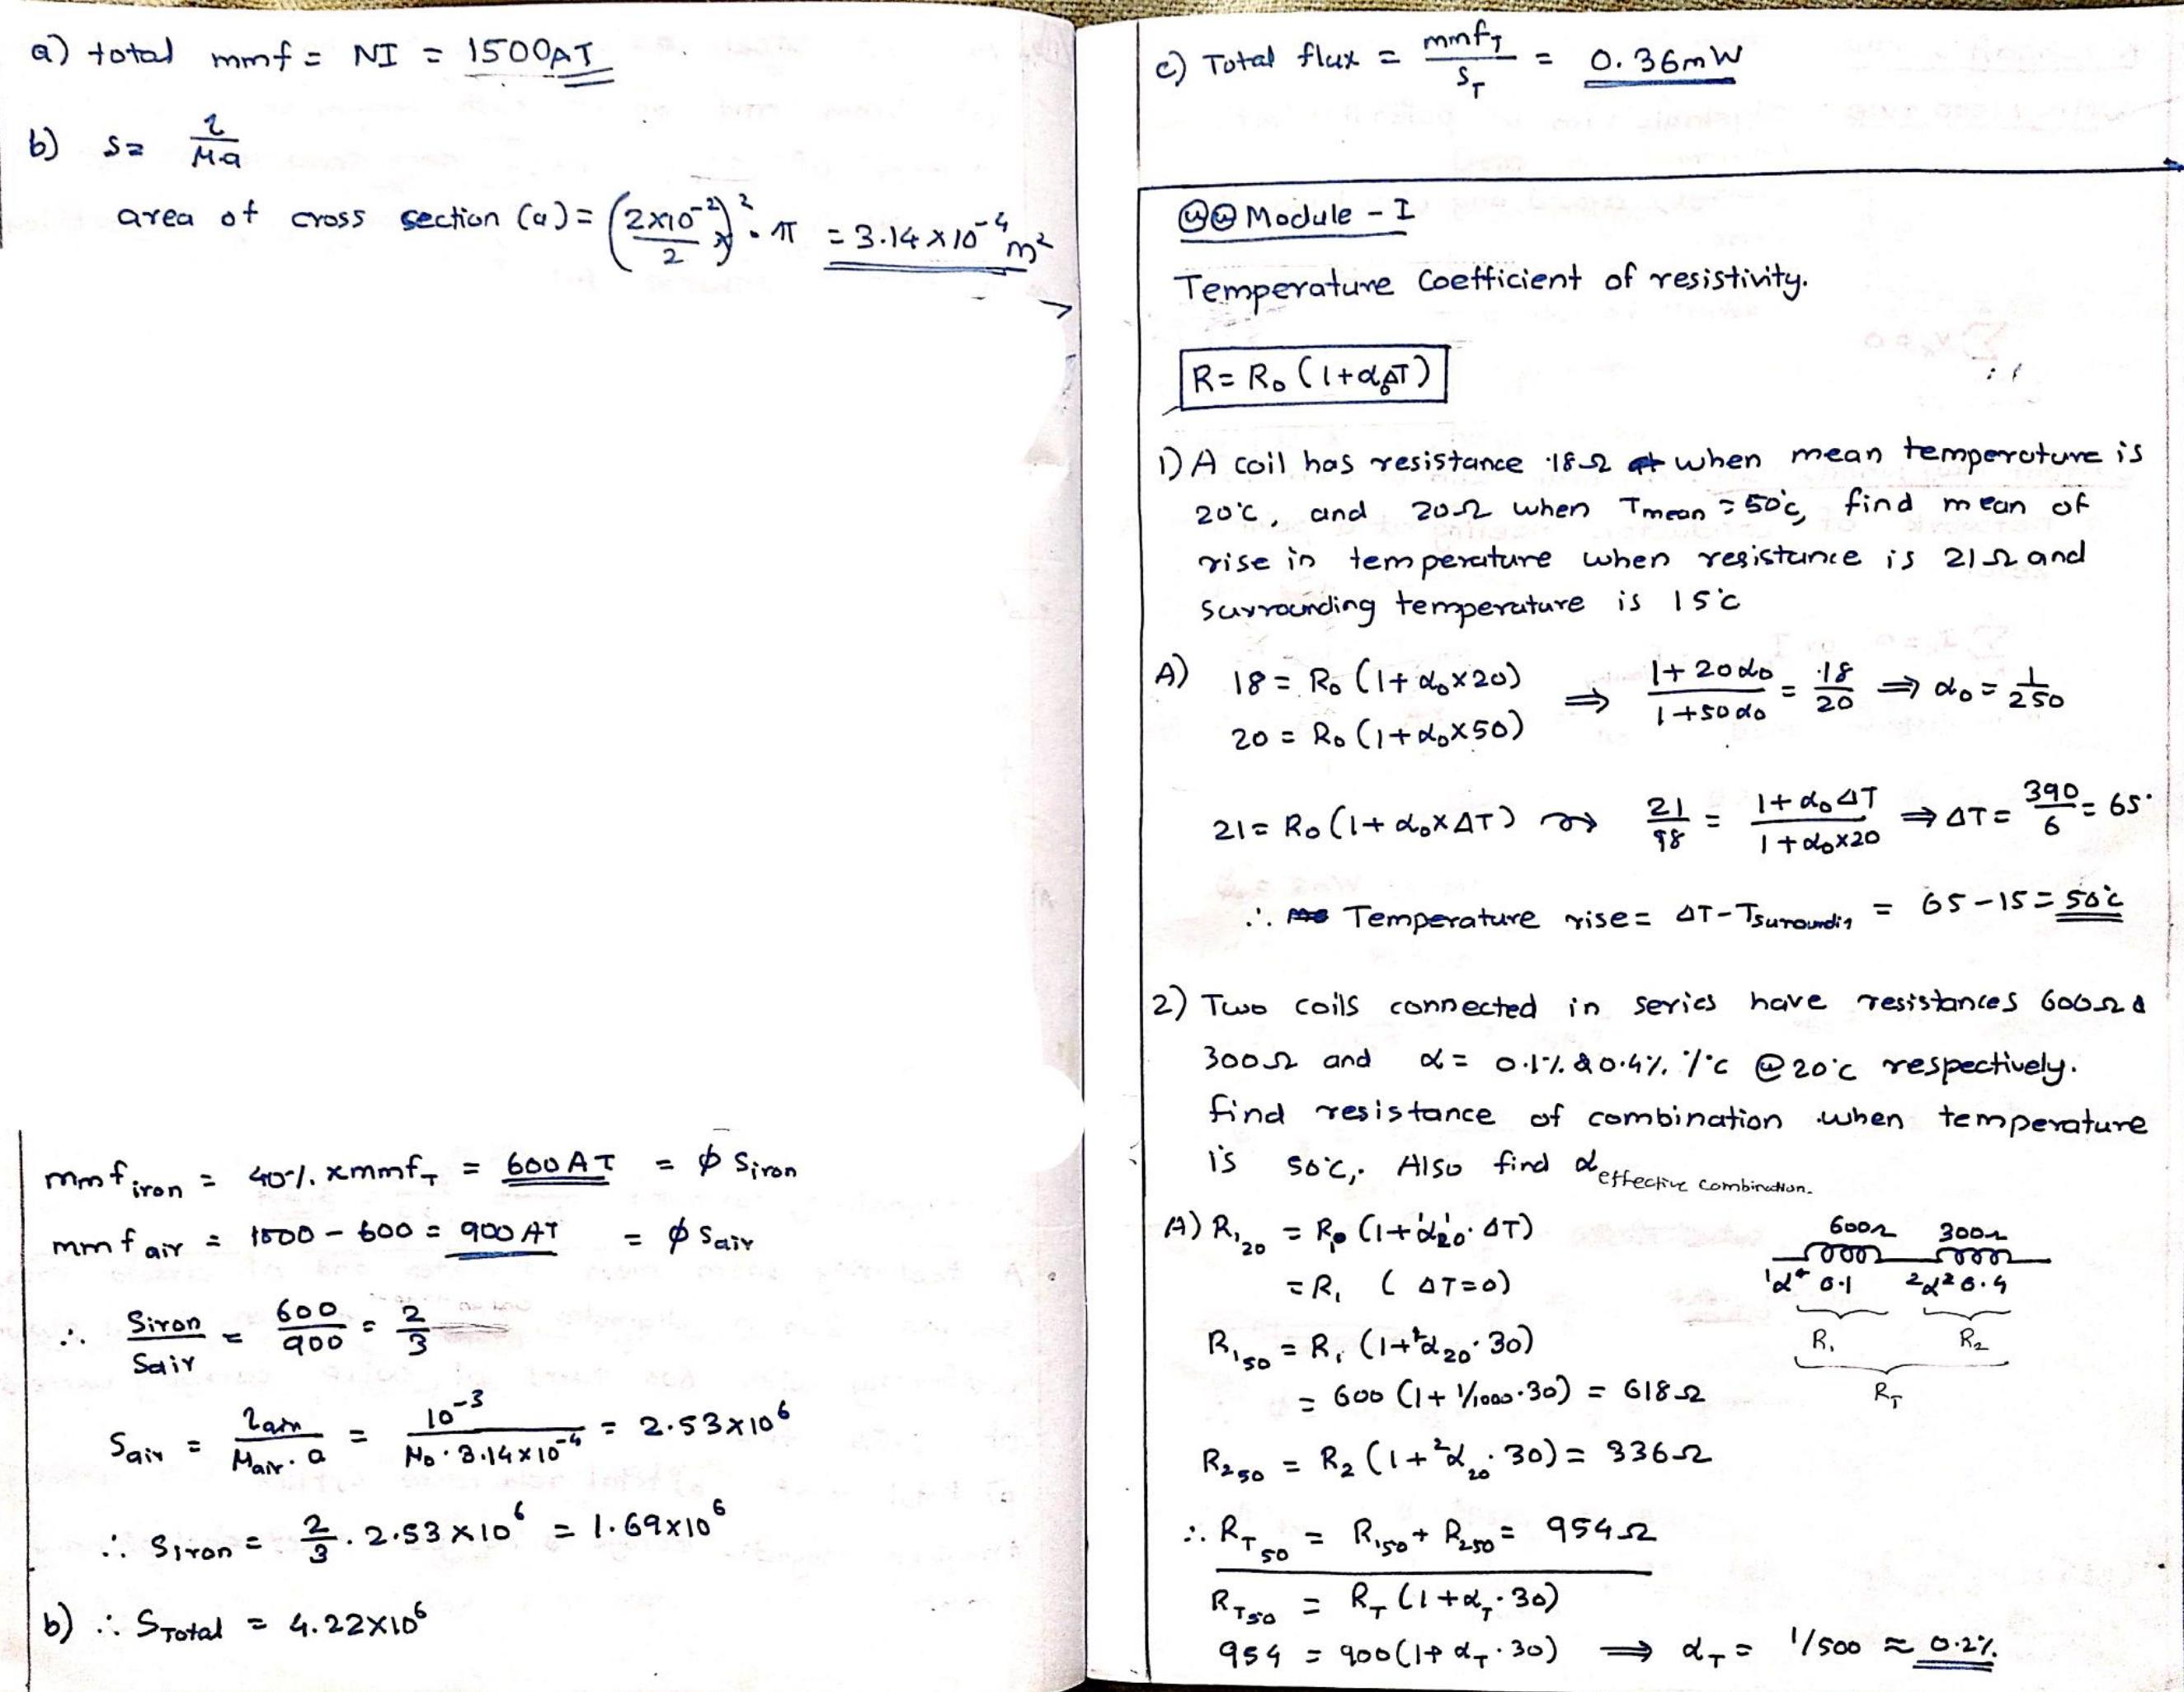
\includegraphics[max width=\figwidth]{2024_06_15_ae1c13e212c06c234cc4g-06}
\end{center}

Kirchhoff's laws

Voltage loop rule: algebraic sum of potential differences 1 directed

(voltage) around any closed loop is zero.

$$
	\sum_{\substack{k=1 \\ n=\infty}}^{n} v_{k}=0
$$

Current law/junctionrale: Algebraic sum of currents in a network of conductors meeting at a point is zero.

$$
	\sum_{k=1}^{n} I_{k}=0 \quad \text { or } I_{\text {entonng }}=I_{\text {leaving }}
$$

$n=$ no. of branches\\
8 III

A cast steel magnetic structure made of a bar of (rose) section, $2 \times 2 \mathrm{~cm}$ is shown in fig. Determine Current That the 500 tum magnetising coil. on the left limb should carry so that a flux of $2 \mathrm{mWb}$ is produced in the right limb. lake $\mu_{r_{\text {steel }}}=600$, neglect leakage\\
A) $\operatorname{mmf}(A T)=N I$

$$
	\begin{aligned}
		 & A T_{B D}=A T_{B C D} .                                                                                                        \\
		 & \therefore A T_{\text {total }}=A T_{A B D A}+A T_{B D}=A T_{D E A B}+A T_{B C D}                                              \\
		 & =\phi S_{B E A B}+\phi_{2} \cdot S_{B C D}                                                                                     \\
		 & \phi_{2}=2 \mathrm{~mW} \text { (given) }                                                                                      \\
		 & \phi_{1} S_{B D}=\phi_{2} S_{B C D}                                                                                            \\
		 & \therefore \phi_{1} \cdot \frac{l_{\infty}}{\mu_{0} \mu_{7} a_{0}}=\phi_{2} \cdot \frac{l_{B c P}}{\mu_{0} H_{2} a}            \\
		 & \eta_{B D}=15 \mathrm{~cm}                                                                                                     \\
		 & \therefore \phi_{1} \cdot \phi_{2} \cdot \frac{e_{B C D}}{e_{B D}}                                                             \\
		 & \tau_{B C D}=25 \mathrm{~cm}                                                                                                   \\
		 & a=2 \times 2 \times 10^{-4} \mathrm{~m}^{2}=4 \times 10^{-4} \mathrm{~m}^{2}                                                   \\
		 & =\phi_{2} \cdot \frac{R S}{15}                                                                                                 \\
		 & =\phi_{2} \cdot \frac{\cdot(0)}{3}=\frac{10}{3} \times 10^{-3} \mathrm{Wm}                                                     \\
		 & \therefore \phi=\phi_{1}+\phi_{2}=2+\frac{10}{3}=\frac{16}{3} \mathrm{~mW}                                                     \\
		 & \therefore A T_{\text {total }}=\phi \cdot S_{D_{G A B}}+\phi_{2} S_{B C D}                                                    \\
		 & =\frac{16}{3} \cdot \frac{2{ }_{D E A B}}{\mu_{0} \mu_{4} \cdot a}+\frac{10}{3} \cdot \frac{2 R_{B \infty}}{\mu_{0} \mu_{2} a}
	\end{aligned}
$$

$$
	\begin{aligned}
		 & \left(\frac{16}{2} \cdot 25+\frac{10}{3} \times .15\right) \frac{10^{-3}}{600 \times 4 \times 10^{-4} \times 4 \pi \times 10^{-7}}=6078 \mathrm{~A} \cdot T \\
		 & A T_{\text {total }}=N \cdot I                                                                                                                              \\
		 & \therefore I=\frac{A T_{\text {tots }}}{N}=\frac{6078.8}{500}=12.16 \mathrm{~A}
	\end{aligned}
$$

Electromagnetic Induction

The phenomenon of producing an emf in a conductor or coil whenever there's a magnetic flux linked with the coil or conductor is known as electromagnetic induction.

Faraday's laws of electromagnetic induction

\begin{enumerate}
	\item Whenever there is a change in the fluxed linked with the coil or conductor, an emf is induced (known as induced emf).
\end{enumerate}

if the coil is closed, a current will flow

\begin{enumerate}
	\setcounter{enumi}{1}
	\item magnitude of induced emf $\alpha$ rate of change is of flux linkage
\end{enumerate}

flux linkage $=N \phi$.

change io flux linkage $=N\left(\phi_{2}-\phi_{1}\right)$

According to Faraday's $2^{\text {nd }}$ law:

$$
	\begin{aligned}
		 & e \propto N\left(\phi_{2}-\phi_{2}\right) / t \quad \\
		 & e=k \cdot(\cdots) \quad k=1 \quad \text { in SI }   \\
		 & e=\frac{N \phi_{2}-N \phi_{1}}{t}
	\end{aligned}
$$

or $e=N \cdot \frac{d \phi}{d t} \quad$ in diff. form

Len 2's law

Induced current will oppose its cause $l$ it will produce a magnetic flux which is opposite to the flux producing a induced current

$$
	e=-N \frac{d \phi}{d t}
$$

Self Inductance

property of a coil which opposes the change in current flowing through it

list method: $\quad e=n \cdot \frac{d \phi}{d t}$. $\frac{d \phi}{d t} \propto \frac{d}{d t}$

charge in I. induces change in flux producing self induced emf

$$
	e=L \frac{d I}{d t}, L=e / \frac{d I}{d t} \quad L=\text { self inductance }
$$

$2^{\text {nd }}$ method:

$$
	\begin{aligned}
		e & =\frac{d}{d t}(N \phi)=\frac{d}{d t}(L I)                    \\
		  & \Rightarrow L=\frac{N \phi}{I} \quad[\text { wb.turns } / A]
	\end{aligned}
$$

III meted:

$$
	\begin{aligned}
		                                     & L=\frac{N \phi}{\Delta I} \Rightarrow \phi=\frac{m m f}{s}=\frac{\phi I}{2 t} \frac{N I}{2 / \mu a}=\frac{N I_{1}}{\tau} \\
		\therefore L=\frac{N^{2} \mu_{a}}{2} & \therefore L=\frac{N^{2} / 4 a}{2}
	\end{aligned}
$$

\begin{enumerate}
	\item A coil wound on an iron core of permeability 400 has 150 turns \& a cross sectional area of $5 \mathrm{~cm}^{2}$ calculate inductance of coil given a steady current of $3 \mathrm{~mA}$ produces a magnetic field of 10 lines $/ \mathrm{cm}^{2}$ where air is present as the medium
\end{enumerate}

A)

$$
	\begin{aligned}
		 & 1 w b=10^{8} \text { lines }                                                                                             \\
		 & \phi=10^{3} \times 5 \times 10^{-4}                                                                                      \\
		 & B=10 \times 10^{-8}=10^{-7} \text { lines } / \mathrm{cm}^{2}                                                            \\
		 & \therefore B\left(\mathrm{wb} / \mathrm{cm}^{2}\right)=400 \times 10^{-7}=4 \times 10^{-5} \mathrm{wb} / \mathrm{cm}^{2} \\
		 & \therefore \phi=B A=4 \times 10^{-5} \times 5=2 \times 10^{-4} \mathrm{hb}                                               \\
		 & L=\frac{N \phi}{I}=\frac{150 \times 2 \times 10^{-4}}{3 \times 10^{-3}}=10 \mathrm{H}
	\end{aligned}
$$

$$
	a=5 \times 10^{-4} \quad \mu_{r}=400
$$

Mutual Inductance

production of in one coil due to flux change in

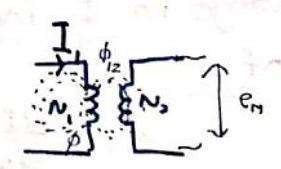
\includegraphics[max width=\textwidth, center]{2024_06_15_ae1c13e212c06c234cc4g-09(1)}\\
other coil.

$$
	e_{M}=N_{2} \cdot \frac{d \phi_{12}}{d t} \equiv M \cdot \frac{d I_{1}}{d b}
$$

or mutual inductance $M=e_{m} / \frac{d I}{d t}$

or

$$
	\begin{aligned}
		e_{m}                            & =N_{2} \frac{d \phi_{12}}{d t}=\frac{d}{d t}\left(N_{2} \phi_{12}\right) \\
		                                 & =m \frac{d I_{1}}{d t}=\frac{d}{d t} \in(m I)                            \\
		\therefore \quad N_{2} \phi_{12} & =m I_{1} \Rightarrow m=\frac{N_{2} \phi_{12}}{I_{1}}
	\end{aligned}
$$

$$
	\phi=\frac{m m f}{s} \quad \therefore \phi_{12}=\frac{N_{1} I_{1}}{2 / \mu a}
$$

$\phi_{12}=\frac{C 1}{4 \mu a}$

$$
	\text { since } \begin{aligned}
		M & =\frac{N_{2} \phi_{12}}{I_{1}} ; M=\frac{N_{1} N_{2} \mu a}{2}=\frac{N_{1} \dot{N}_{2}}{S} \\
		  & =\frac{N_{2} N_{1} I_{1} \mu a}{2 I_{1}} ;
	\end{aligned}
$$

$\therefore$ Inductance

self (L)

$e / \frac{d I}{d t}$

$\frac{\text { mutual }(M)}{e_{n} / \frac{d I}{d t}}$

$$
	\frac{N_{2} \phi_{12}}{I} \quad \because I_{2}
$$

\begin{center}
	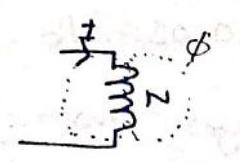
\includegraphics[max width=\figwidth]{2024_06_15_ae1c13e212c06c234cc4g-09(2)}
\end{center}

$\frac{N^{2} \mu 9}{2}$

$w^{2} / 5$

$$
	\begin{aligned}
		 & \frac{N_{1} N_{2} \mu a}{2} \\
		 & N_{1} N_{2} / s
	\end{aligned}
$$

Coefficient of Coupling ( $k$ )

\begin{center}
	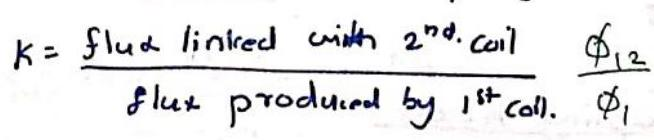
\includegraphics[max width=\figwidth]{2024_06_15_ae1c13e212c06c234cc4g-09(3)}
\end{center}

\begin{center}
	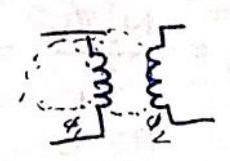
\includegraphics[max width=\figwidth]{2024_06_15_ae1c13e212c06c234cc4g-09}
\end{center}

$\phi_{12}=k \phi_{1}=$ A mount of flax produced in first ail linking with $2^{\text {nd }}$ coil.

$$
	\begin{aligned}
		 & M_{12}=\frac{N_{2} k \phi_{12}}{I_{1}}, M_{21}=\frac{N_{1} k \phi_{21}}{I_{2}}, L_{1}=\frac{N_{1} \phi_{1}}{I_{1}} \quad L_{2}=\frac{N_{2} \phi_{2}}{I_{2}} \\
		 & \text { so } M_{12}=M_{21}=m                                                                                                                                \\
		 & \therefore M_{12} \cdot M_{21}=\frac{k^{2} N_{1} M_{2} \cdot \phi_{1} \phi_{2}}{I_{1} I_{2}}=k^{2} L_{1} L_{2}=m^{2}                                        \\
		 & \therefore \quad M=K \sqrt{L_{1} L_{2}}
	\end{aligned}
$$

$$
	\text { or } K=\frac{M}{\sqrt{L_{1} L_{2}}}
$$

\begin{enumerate}
	\item Two identical coits $A, B$ of 1000 turns is ewit lying parallel planes such that $80 \%$ of flux produced by one coil links with the other $A$ current of $5 \mathrm{~A}$ flowing in coil $A$ produces a flax of $0.05 \mathrm{mWb}$ is it. If the current in the coil $A$ changes from $412 A$ to $-12 A$ in 0.023 . Calculcutr i) mutual indudane Ti) emf indused in coil 'B.
\end{enumerate}

A) $I_{A}=S A, \quad \phi_{A}=0.05 m W, \quad N=1000$

\begin{center}
	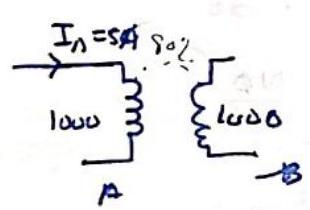
\includegraphics[max width=\figwidth]{2024_06_15_ae1c13e212c06c234cc4g-10}
\end{center}

$\therefore L_{A}=\frac{N_{1} \phi_{1}}{I_{1}}=\frac{1000 \times 0.05 \times 10^{-3}}{5}$

Coils $A$ \& $B$ in a magnetic circuit havee $600 \$ 500$ turns respectively, $A$ carrent of $8 A$ in coil $A$ produces a flux of $0.04 w b$. If $k=0.2$, calculate

	i) Self inductance of $A$ iii) Avg.emf induced in $B$ ii) flux linking with coil B \& flux with it changes from

	iv) mutual inductance

	v) Avg emf in $B$ when $I_{A}$ changes from o to \&A in 0.055

	Aji)Self inductance $=\frac{M \phi_{A}}{I_{A}}$

	ii) flux linked $\phi_{B}=k . \phi_{A}=0.2 \times 0.04=0.008 \mathrm{WB}=8 \mathrm{mWb}$\\
	i) $M_{A B}=\frac{N_{2} \Phi_{12}}{I_{1}}=\frac{1000 \times 0.0 \$ \times 10^{-3}}{5}=$

	$$
		\text { - } \varepsilon_{B}=N \frac{\Delta \phi}{\Delta t}=500 \times \frac{8 \mathrm{mWb}-0}{0.025}=\operatorname{so0} \times \frac{0.008}{0.02}=200
	$$

	iv) $M=\frac{N_{2} \phi_{12}}{I_{1}}=\frac{N_{B} \phi_{B}}{I_{A}}=\frac{500 \times 8 \times 10^{-3}}{8}=0.51 \mathrm{H}$

	v) When $I_{A} \in[0,8]$


	\begin{align*}
		           & \phi_{A} \in[0,40 \mathrm{mWb}], \phi_{B} \in[0,8 \mathrm{mWb}]                                           \\
		\therefore & \varepsilon_{B}=N \frac{d \phi_{B}}{d q}=500 \cdot \frac{8 \mathrm{mWb}-0}{0.05}=500 \frac{0.008}{0.05} .
	\end{align*}


	ii) emf incluced $=m \cdot \frac{d I}{d t}=m \frac{(12+12)}{0.02}$

$\rightarrow M \cdot \frac{d L}{d t}=0.5 \times \frac{8}{0.05}=\dot{i}$

	Inductance in series
	$$
		L_{e q}=\left\{\begin{array}{l}
			\sum_{v_i} L_i, \text { wo mutual inductance } \\
			L_1+L_2+2 m, \text { w. mut. } E(\omega \cdot 2 L) .
		\end{array}\right.
	$$
	$$
		\begin{gathered}
			\text { fluxes are } \\
			\text { "aiding" } \\
			L_1+L_2+2 m
		\end{gathered}
	$$
	Recons
$+855$
	Inductance in parallel
	$$
		\begin{aligned}
			 & L_{\text {eq }}=\sum_{v_1} L_{U_{(2)}} \omega / 0 \\
			 & L_{e q}=\frac{4 L_2-M^2}{L_1+L_2-\omega 2 M}      \\
			 & L_{e q .}=\frac{L_1 L_2-M^2}{L_1+L_2+2 M}
		\end{aligned}
	$$
	$$
		w / 0 \cdot M \cdot I
	$$
	fluxes are aiding

	Energy stored: $\frac{1}{2} L I^2$
	AC-fundtamentals
	$$
		v=V_m \sin (\omega t), i=I_m \sin (\omega t)
	$$

	Advantages of sing.
	1) Sinosoiclal signels produce less disturbance to elect. network compared with other generateling signals and the waveform is smooth and efficient
	2) Sinusoidal signals applied to appropriately designed colils can produce a revolving field that can do the work.
	3) mathematical calculations associated with a sinosoidal signals are much simpler
	9). with the hap of fourier series, any alternating signal can be represented os the sum of different sinosoidal signals.

	Parameters to represent alternating signal
	1) Peak value 〜 Amplitude
	2) peak to peak $\sim V_{p p}$ ?
	3) Average value. $/ D C$ value.
	$$
		=\frac{1}{T_0} \int_0^T f(t) d t
	$$
	for symmetric, take $1 / 2$ cycle. $\equiv \frac{2}{T} \int_0^{T / 2} f(t) d t$
	e.y: $\frac{2}{2 \pi} \int_0^\pi v_m \sin (u t) d a t=\frac{a}{\pi}\left(2 v_m\right)^0=\frac{2}{\pi} v_m$


	1.
	$$
		\begin{aligned}
			 & =25 \mathrm{~V} \\
			 &
		\end{aligned}
	$$
	2 Area under cure
	$$
		\begin{aligned}
			= & \frac{10 \times 0.2}{2}+0.4 \times 10+\frac{0.2 \times 10}{2} \\
			  & -\frac{0.2 \times 5}{2}                                       \\
			= & 6.5
		\end{aligned}
	$$
	$$
		\therefore \text { Aug val }=\frac{6.5}{1}=\underline{6.5 V}
	$$
	3. FWR:
	$$
		\begin{aligned}
			\text { Aug. val } & =\frac{1}{\pi} \int_0^\pi \sin (\theta) d \theta \\
			                   & =\frac{\pi}{\pi}[-\cos \theta]_0^\pi             \\
			                   & =\frac{\pi}{\pi}(n)=0 . \pi 1
		\end{aligned}
	$$
	4. H'wR
	$$
		\begin{aligned}
			\text { Avg val } & =\frac{1}{2 \pi} \int_0^\pi \sin (\theta) d \theta \\
			                  & =\frac{1}{\pi}
		\end{aligned}
	$$

	FWR, HWR wave.
	RMS value.
$\sim$ Rms value of on alternating current is thad steady current (dc current) flowing through a given resista for a given time which produces same heating effect as \& by the a AC for the same resistance for the same tires. time
	Here tola heating effect
	$$
		\begin{aligned}
			 & I \simeq \underbrace{\sqrt{\frac{1}{N} \sum_{k=1}^N i_{15}^{m=m^2}}}_{\text {root mew square }} \\
			 & I=\sqrt{\frac{1}{T} \int_0^T i(t)^2 d t}                                                        \\
			 &
		\end{aligned}
	$$
	for symmetric wave: $R_{m s}=\sqrt{\frac{s q \cdot a v 0 \text { of } 1 / 2 c_y}{1 / 2 T}}$.
	for sin.
	$$
		\text { - form factor } \begin{aligned}
			                            & =\frac{v_{r m s}}{v_{a v g}}                                             \\
			\text { for } \sin H \omega & =\frac{v_m}{\sqrt{2}} \cdot \frac{\pi}{2 v_m}=\frac{\pi}{\sqrt{8}}=1.111 \\
			\text { - Peak factor }     & =\frac{v_m}{v_{r m s}}=v_m / \frac{v_m}{\sqrt{2}}=\sqrt{2}=1.414
		\end{aligned}
	$$

	1.

	$$
		\begin{aligned}
			A_{\text {vg. Val }} & =\frac{100 \times .5 \bar{\Phi} 50 \times .5}{1} \\
			                     & =25 \mathrm{~V}
		\end{aligned}
	$$

	\begin{center}
		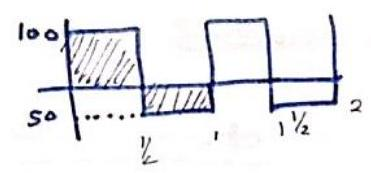
\includegraphics[max width=\figwidth]{2024_06_15_74bbabba7981675b0d49g-01(1)}
	\end{center}

	2 Area under cure

	$$
		\begin{aligned}
			 & =\frac{10 \times 0.2}{2}+0.4 \times 10+\frac{0.2 \times 10}{2} \\
			 & -\frac{0.2 \times 5}{2}                                        \\
			 & =6.5
		\end{aligned}
	$$

	$$
		\therefore \text { Aug val }=\frac{6.5}{1}=6.5 V
	$$

	\begin{enumerate}
		\setcounter{enumi}{2}
		\item FWR:
	\end{enumerate}

	Aug. val $=\frac{1}{\pi} \int_{0}^{\pi} \sin (\theta) d \theta$

	$$
		\begin{aligned}
			 & =\frac{\pi}{\pi}[-\cos \theta]_{0}^{\pi} \\
			 & =2 / \pi                                 \\
			 & \pi(2)=0.64
		\end{aligned}
	$$

	\begin{enumerate}
		\setcounter{enumi}{3}
		\item H'wR
	\end{enumerate}

	$$
		\begin{aligned}
			\frac{H w R}{A v g} \text { val } & =\frac{1}{2 \pi} \int_{0}^{\pi} \sin (\theta) d \theta \\
			                                  & =\frac{1}{\pi} \quad=0 . B R
		\end{aligned}
	$$

	\begin{center}
		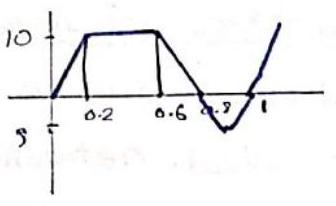
\includegraphics[max width=\figwidth]{2024_06_15_74bbabba7981675b0d49g-01(4)}
	\end{center}

	FWR, HWR wave.

	\begin{center}
		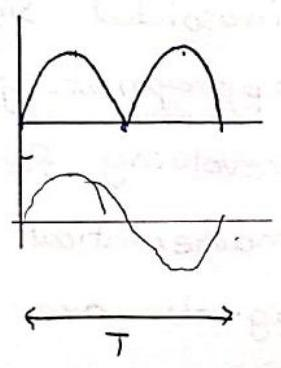
\includegraphics[max width=\figwidth]{2024_06_15_74bbabba7981675b0d49g-01(3)}
	\end{center}

	$$
		\begin{aligned}
			 & I=\underbrace{\sqrt{\frac{1}{N} \sum_{k=1}^{N} i_{15}^{m_{m}^{2}}}}_{\text {root mew square }} \\
			 & I=\sqrt{\frac{1}{T} \int_{0}^{T} i(t)^{2} d t}
		\end{aligned}
	$$

	for symmetric wave: $R_{m s}=\sqrt{\frac{s q \cdot a 00011 / 2 c y}{1 / 2 T}}$.

	for sin.

	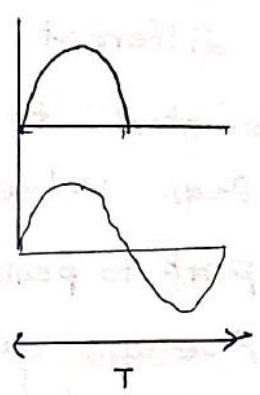
\includegraphics[max width=\textwidth, center]{2024_06_15_74bbabba7981675b0d49g-01}\\
	the same tire time

	Here total heating effect

	\begin{center}
		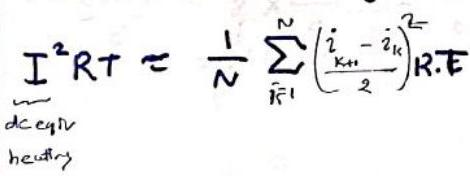
\includegraphics[max width=\figwidth]{2024_06_15_74bbabba7981675b0d49g-01(2)}
	\end{center}

	RMS value.

$\sim$ Rms value of on alternating current is shad steady current (dc current) flowing through a given resista for a given time which produces same heating effect as by the a AC for the same resistance for

	\begin{center}
		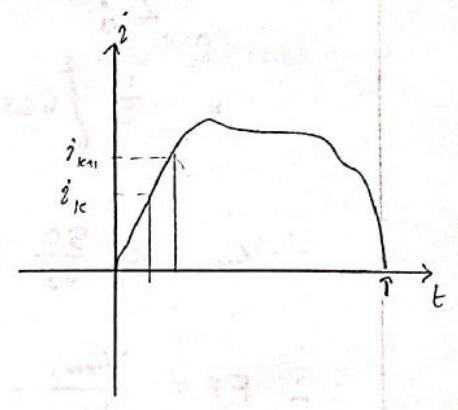
\includegraphics[max width=\figwidth]{2024_06_15_74bbabba7981675b0d49g-01(5)}
	\end{center}

	$$
		\begin{aligned}
			 & J_{v n s}=\sqrt{\frac{1}{2 \pi} \int_{0}^{2 \pi} v_{m}^{2} \sin ^{2}(\theta) d \theta}=                                                                                                             \\
			 & =\sqrt{\frac{V_{m}^{2}}{2 \pi} \int_{0}^{2 \pi}\left(\frac{1}{2}-\frac{\cos (2 \theta)}{2}\right)} d \theta=\sqrt{\frac{V_{m}^{2}}{4 \pi}\left[\theta-\frac{\sin (2 \theta)}{2}\right]_{0}^{2 \pi}} \\
			 & =\sqrt{\frac{v_{m}^{2}}{4 \pi}(2 \pi)}=\frac{v_{m}}{\sqrt{2}}
		\end{aligned}
	$$

	\begin{itemize}
		\item form factor $=\frac{V_{\text {rms }}}{V_{\text {avg }}}$
	\end{itemize}

	for $\sin H \omega=\frac{v_{m}}{\sqrt{2}} \cdot \frac{\pi}{2 v_{m}}=\frac{\pi}{\sqrt{8}}=1.111$

	\begin{itemize}
		\item Peak factor $=\frac{v_{m}}{v_{r m s}}=v_{m} / \frac{v_{m}}{\sqrt{2}}=\sqrt{2}=1.414$

		\item RmS of $F W R, T=\pi \quad H W R \quad T=2 \pi$

	\end{itemize}

	RMS of a complex ware

	\begin{enumerate}
		\item find FF of given waveform
	\end{enumerate}

	A)

	$$
		\begin{aligned}
			V_{\text {Avg }}     & =\frac{50 \times 2}{4}=25 V                                                                                                                \\
			V_{r m s}^{2}        & =\frac{1}{T} \int_{0}^{T} v(t) d b                                                                                                         \\
			                     & =\frac{1}{2} \int_{0}^{2}(25 t)^{2} d t                                                                                                    \\
			                     & =\frac{1}{2} \int_{0}^{2} 625 t^{2} d t=\frac{625}{2}\left[\frac{t^{3}}{3}\right]_{0}^{2}=\frac{625}{6} \times 8=\frac{4 \times 25^{2}}{3} \\
			\therefore V_{r m s} & =\frac{50}{\sqrt{3}}=\underline{28.87 V}                                                                                                   \\
			\therefore F F       & =\frac{V_{r m s}}{V_{v u v}}=\frac{28.87}{25}=1.155
		\end{aligned}
	$$

	\begin{center}
		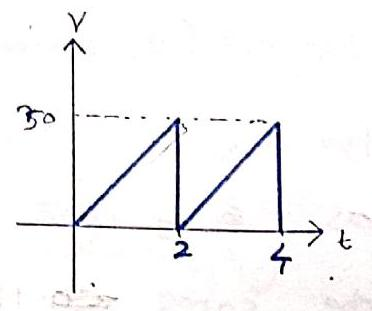
\includegraphics[max width=\figwidth]{2024_06_15_74bbabba7981675b0d49g-02(1)}
	\end{center}

	\begin{enumerate}
		\setcounter{enumi}{1}
		\item $V_{\text {Avg }}=0$ ? 1
	\end{enumerate}

	$$
		\begin{aligned}
			V_{\text {RmS }}^{2}         & =\frac{1}{1} \int_{0}^{1}(4 t-2)^{2} d t=\int_{0}^{1}\left(16 t^{2}+4-18 t\right) d t \\
			                             & 0                                                                                     \\
			                             & =\left[8 \frac{16 t^{3}}{3}+4 t-8 t^{2}\right]_{0}^{1}=\frac{16}{3}+4-8=\frac{4}{3}   \\
			\therefore V_{\text {Taos }} & =\frac{2}{\sqrt{3}}=1.155
		\end{aligned}
	$$

	\begin{center}
		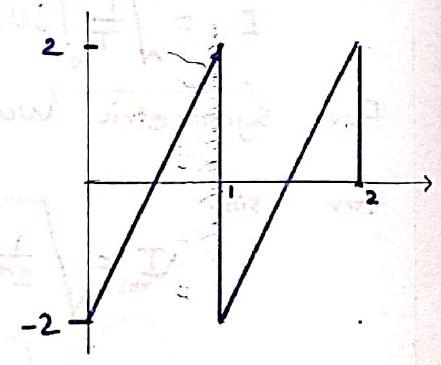
\includegraphics[max width=\figwidth]{2024_06_15_74bbabba7981675b0d49g-02}
	\end{center}

	\begin{itemize}
		\item Every alternating sign waveform can be representol completely if we hove.
	\end{itemize}

	i) Amplitade ii) frequency iii) phase difference phasor representation

	VAF arert scalu nor vec but phasor-\\
	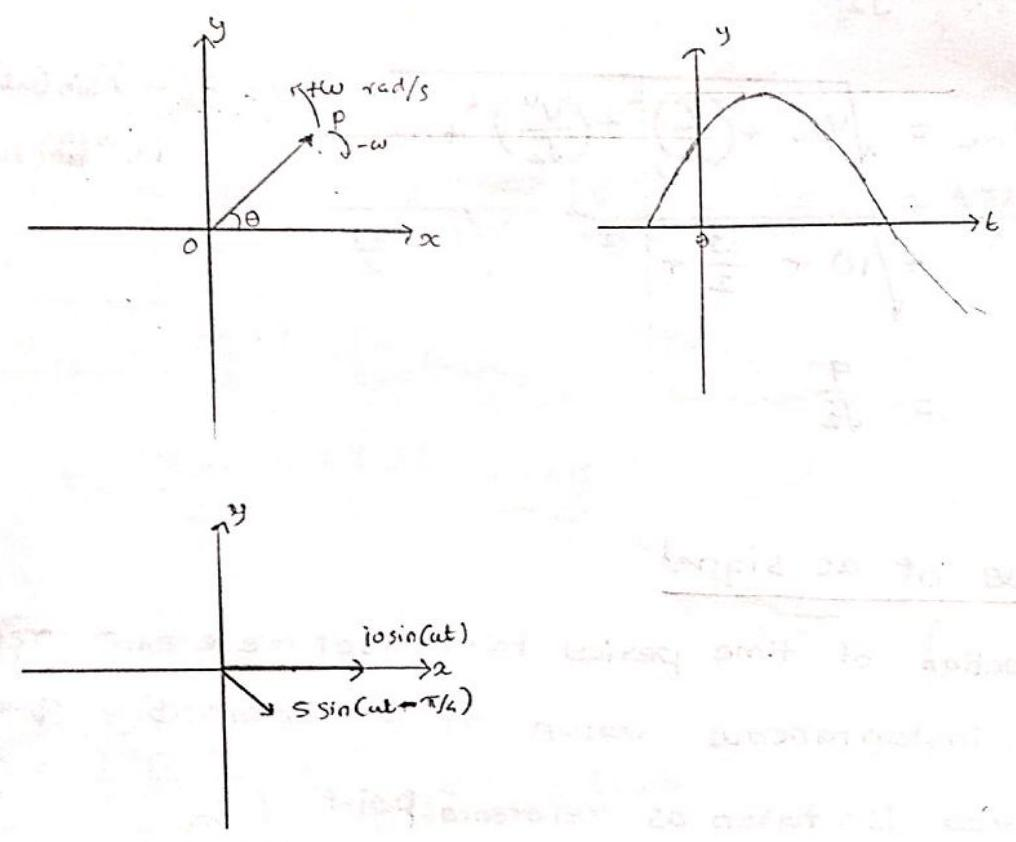
\includegraphics[max width=\textwidth, center]{2024_06_15_74bbabba7981675b0d49g-03(3)}

	Addition of phasors

$o c=\sqrt{o p^{2}+\rho c^{2}}$

$=\sqrt{\left(0 p^{\prime}+p^{\prime} p\right)^{2}+p c^{2}}$

$=\sqrt{(|A|+|B| \cdot \cos (\theta))^{2}+(|B| \cdot \sin (\theta))^{2}}$

$=\sqrt{|A|^{2}+|B|^{2}+2|A||B| \cdot \cos (\phi)}$

	\begin{center}
		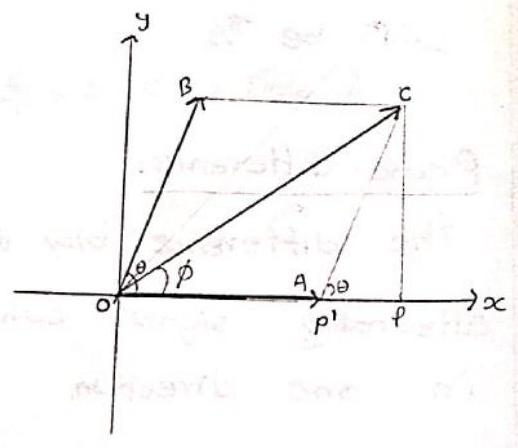
\includegraphics[max width=\figwidth]{2024_06_15_74bbabba7981675b0d49g-03(1)}
	\end{center}

$\phi=\tan ^{-1} \frac{|B| \sin (\theta)}{|A|+|B| \cos (\theta)}$ methud of components.

	\begin{center}
		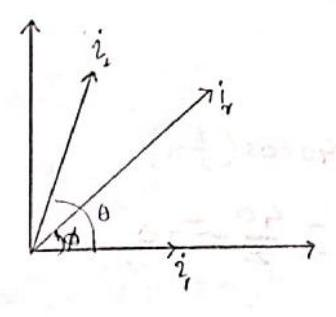
\includegraphics[max width=\figwidth]{2024_06_15_74bbabba7981675b0d49g-03}
	\end{center}

	Split phasor to $x, y$ camponents.

$\therefore$ Resultant $=\sqrt{x^{2}+y^{2}}$

$i_{1}(x)=i_{1}, i_{1}(y)=0$

$\dot{i}_{2}(x)=\dot{i}_{2} \cos (\theta), i_{2}(y)=\dot{z}_{2} \sin (\theta)$

$\begin{aligned} \phi=\tan ^{-1}\left(\frac{x}{g}\right)=\tan \left(\frac{\dot{z}_{2} \sin (\theta)}{\left.z_{1}+i_{2}^{2} \cos \theta\right)}\right) \dot{i}_{\gamma} & =\sqrt{\left(i_{1}+\dot{i}_{2} \cos (\theta)\right)^{2}+\left(0+\dot{i}_{2} \sin (\theta)\right)^{2}} \\ & =\sqrt{\dot{i}_{1}^{2}+\dot{i}_{2}^{2}+2 \dot{i}_{1} \dot{z}_{2} \cos (\theta)}\end{aligned}$

$\Leftrightarrow$

	Three circuils in parallel take the follouing currens

$i_{1}=20 \sin (314 t), i_{2}=30 \sin (314 t-\pi / 4), i_{3}=40 \cos \left(314 t+\frac{\pi}{6}\right)$

	find

	i) expression for resultant current

	ii) its rms value and frequency.

	iii) If the circuit has a resistarce of $2 \Omega$ what is the enorgy loss in lohour

	A) $i_{2}=40 \sin \left(314 t+\frac{\pi}{2}+\frac{\pi}{6}\right)$

$=40 \sin \left(314 t+\frac{2}{3} \pi\right)$

$\dot{z}$

	i

$i$

	\begin{center}
		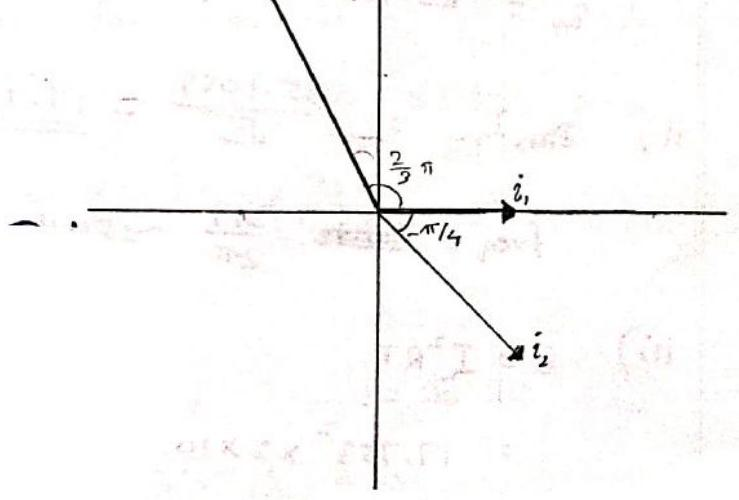
\includegraphics[max width=\figwidth]{2024_06_15_74bbabba7981675b0d49g-03(2)}
	\end{center}

	Phasor algebra (『)

	$$
		\begin{aligned}
			\odot \vec{B} & =j^{2} \vec{A} \\
			\vec{C}       & =j \vec{A}
		\end{aligned}
	$$

	$$
		\begin{aligned}
			 & i_{1}(x)=20, \quad i_{2}(x)=30 \cos (-\pi / 4) \quad i_{3}(x)=40 \cos \left(\frac{2}{3} \pi\right)                        \\
			 & =\frac{30}{\sqrt{2}} \quad=-\frac{40}{2}=-20                                                                              \\
			 & \therefore \dot{z}_{r}(x)=20+\frac{30}{\sqrt{2}}-20=\frac{30}{\sqrt{2}}                                                   \\
			 & i_{2}(y)=0 \quad \dot{i}_{2}(y)=30 \sin (-\pi / 4), i_{3}(y)=40 \sin \left(\frac{2}{3} \pi\right)                         \\
			 & =-\frac{30}{\sqrt{2}} \quad=40 \cdot \text { 蒌 } \frac{\sqrt{3}}{2}                                                       \\
			 & \therefore \dot{i}_{7}(y)=40 \frac{\sqrt{3}}{2}-\frac{30}{\sqrt{2}}=\frac{40 \sqrt{6}-30 \sqrt{2}}{2}                     \\
			 & \therefore\left|\dot{i}_{r}\right|=\sqrt{\dot{i}_{r}(x)^{2}+\dot{i}_{r}(y)^{2}}=\sqrt{\frac{900}{2}+(\cdots)^{2}}=25.1059 \\
			 & \theta=\frac{\eta_{r}(y)}{i_{r}(x)} \tan ^{1} \theta=32.3^{\circ}
		\end{aligned}
	$$

	$$
		\therefore i_{r}=25.1059 \sin \left(314 t+32.3^{\circ}\right) \mathrm{A}
	$$

	ii) حreos $I_{r m s}=\frac{25.1059}{\sqrt{2}}=17.753 \mathrm{~A}$

	$$
		f_{\text {req }}=\frac{314}{2 \pi} \simeq 50 \mathrm{~Hz}
	$$

	iii).

	$$
		\begin{aligned}
			E & =I_{m}^{2} R T                                                       \\
			  & =17.753^{2} \times 2 \times 10 \times 60 \times 60=22.69 \mathrm{MJ} \\
			  & =17.753^{2} \times 2 \times 10^{710^{-9}}=6.303 \mathrm{kwh}
		\end{aligned}
	$$

	$$
		\begin{aligned}
			             & =4000\left(\cos (\pi / 4-\pi / 6)+\cos \left(2 \omega t+\frac{\pi}{4}+\frac{\pi}{6}\right)\right)                                                      \\
			P            & =4000\left(\cos \left(\frac{\pi}{12}\right)+\cos \left(2 \omega t+\frac{5}{12} \pi\right)\right)                                                       \\
			\therefore P & =\int_{0}^{\pi / 50} 4000\left(\cos \frac{\pi}{12} \%+\cos \left(2 \omega t+\frac{5}{12} \pi\right)\right) d t                                         \\
			             & =4000 \times \frac{\pi}{50} \cos \frac{\pi}{12}+\left[\frac{\sin \left(2 \omega t+\frac{5}{12} \pi\right)}{2 \omega} \times 4000\right]_{0}^{\pi / 50} \\
			             & =80 \pi \cos \pi / 12                                                                                                                                  \\
			             & =\frac{242.76}{=}
		\end{aligned}
	$$

	2 phosors are given in the rectangle form as: $\eta_{1}=(15+10 j) A$ ard $\eta_{2}=(12+6 j) A$, perform $\eta_{1}+\eta_{2}$ and $\eta_{1}-\eta_{2}$\\
	A) $z_{1}+\eta_{2}=26+16 j, \quad \eta_{1}-\eta_{2}=3+4 j$

	\begin{enumerate}
		\setcounter{enumi}{2}
		\item Determine the resultant voltage of two sinosoidal generators in series whose voltages are, $v_{1}=25 \angle 15^{\circ} \mathrm{V}, v_{2}=15<60^{\circ} \mathrm{V}$
	\end{enumerate}

	A)

	$$
		\begin{aligned}
			 & v_{1}(x)=25 \cos \left(15^{\circ}\right), \quad v_{2}(x)=15 \cos ^{3}\left(60^{\circ}\right) \\
			 & v_{1}(y)=25 \sin \left(15^{\circ}\right) \quad u_{2}(y)=15 \sin \left(0^{\circ}\right)       \\
			 & R(x)=                                                                                        \\
			 & |R|=85)=19.46                                                                                \\
			 &                                                                                              \\
			 & \therefore R=37.15<31.59^{\circ}
		\end{aligned}
	$$

	AC circuits

	Pure resistive circuit

$V=V_{m} \sin (\omega t)$

	\begin{center}
		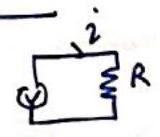
\includegraphics[max width=\figwidth]{2024_06_15_74bbabba7981675b0d49g-05(1)}
	\end{center}

	Q inst. caners. valise

	. ins .t. current:

	$$
		\begin{aligned}
			i & =\frac{V_{m}}{R} \sin (\omega t) \\
			  & :=N / R
		\end{aligned}
	$$

	\begin{center}
		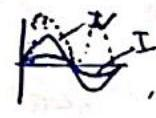
\includegraphics[max width=\figwidth]{2024_06_15_74bbabba7981675b0d49g-05}
	\end{center}

	Here both voltage \& current case in phase.

	Instantaneous power $=v \cdot i$

	$$
		\begin{gathered}
			=\frac{v_{m}^{2}}{R} \sin ^{2}(\omega t) \\
			=\frac{V_{m} I_{m}}{2}-\frac{V_{m} I_{m} \cos (2 \omega t)}{2}
		\end{gathered}
	$$

	\begin{center}
		\includegraphics[max width=\figwidth]{2024_06_15_74bbabba7981675b0d49g-05(3)}
	\end{center}

	$$
		=\frac{V_{m} I_{n}}{2}=\frac{V_{m}}{\sqrt{2}} \frac{I_{m}}{\sqrt{2}}=\underline{\underline{V I}} \text { Rms values. }
	$$

	Purely inductive circuit

	\begin{center}
		\includegraphics[max width=\figwidth]{2024_06_15_74bbabba7981675b0d49g-05(2)}
	\end{center}

	$$
		\begin{aligned}
			v            & =v_{m} \sin (\omega t)                                                                                                                                                                    \\
			             & =v_{i}=L \frac{d i}{d t}                                                                                                                                                                  \\
			\therefore i & =\int \frac{v_{L}}{L} d t=\frac{V_{m}}{\omega L} \cos ^{2}(\omega t)=\frac{v_{m}}{L \omega} \cdot \sin \left(\omega t-\frac{\pi}{2}\right)=I_{m} \sin \left(\omega t-\frac{\pi}{2}\right)
		\end{aligned}
	$$

	\begin{center}
		\includegraphics[max width=\figwidth]{2024_06_15_74bbabba7981675b0d49g-05(4)}
	\end{center}

$\therefore i$ is ben lagging behind $V$ ben

	$$
		\begin{aligned}
			 & I_{m}=\frac{v_{m}}{\omega L} \therefore \frac{\dot{V}_{m}}{I_{m}}=\omega L=2 \pi f L=X_{c}      \\
			 & \therefore G=\frac{1}{x_{C}}=\frac{1}{\omega L}=\frac{1}{2 \pi f L}=B_{L} \text { susceptanco }
		\end{aligned}
	$$

	Instantaneous power : $p=V_{i}$

	$$
		\begin{aligned}
			P & =V_{i}                                                                                  \\
			  & =V_{m} J_{m} \sin (\omega t) \sin \left(\omega t-\frac{\pi}{2}\right)                   \\
			  & =\frac{U_{m} I_{n}}{2} \cdot 2 \sin (\omega t) \sin \left(\omega t-\frac{\pi}{2}\right)
		\end{aligned}
	$$

	$$
		\begin{aligned}
			 & =\frac{V_{m} I_{m}}{2}[-2 \sin (\omega t) \cos (\omega t)] \\
			 & =-\frac{V_{m} I_{m}}{2} \sin (2 \omega t)
		\end{aligned}
	$$

$\therefore$ Avg. Power $=\frac{1}{2} \frac{1}{\pi} \int_{0}^{2 \pi}-\frac{V_{m} I_{m}}{2} \sin (2 \omega t) d t$

	$$
		=\frac{1}{2 \pi}\left[\frac{y_{m} I_{m}}{2 \times 2 \omega} \cdot \cos (\omega t)\right]_{0}^{2 \pi}=0
	$$

$\therefore$ no power is consumed in purely inductive resistance

	Purely capacitive circuit

	$$
		v=v_{m} \sin (\omega t)
	$$

	Instantaneous charge shred:

	$$
		\begin{aligned}
			q & =C v                           \\
			  & =C \cdot v_{m} \sin (\omega t)
		\end{aligned}
	$$

	\begin{center}
		\includegraphics[max width=\figwidth]{2024_06_15_74bbabba7981675b0d49g-06}
	\end{center}

$\therefore$ inst .t. current: $i=\frac{d a}{d t}=C \omega v_{m} \cos (\omega t)=C \omega \cdot v_{m} \sin \left(\omega t+\frac{\pi}{2}\right)$

	$$
		\begin{aligned}
			\frac{V_{m}}{I_{m}}=\frac{1}{\omega C} & =\frac{1}{2 \pi f c}=x_{c}-\text { (capacitive reactances) } \\
			\frac{1}{x_{c}}                        & =\omega \cdot C=B_{c} \text { - (apacitive susceptance. }
		\end{aligned}
	$$

	Instantaneous power: $p=v i=v_{m} I_{m} \sin (\omega t) \cos (\omega t)$

	$$
		=\frac{V_{m} I_{m}}{2} \sin (2 \omega t)
	$$

	Average power $=\frac{1}{2 \pi} \int_{0}^{2 \pi} \frac{V_{m} I_{m}}{2} \sin (2 \omega t) d t=0$

$\therefore$ Here no power drawn

	\begin{enumerate}
		\item A pure inductive coil allows a current of $\operatorname{LOA}$ to flow from a $230 V 50 H_{2}$ supply. rms find $x_{C}, L$, power absorbed, $i(t)=$ ? $v(t)=$ ?
	\end{enumerate}

	A))

	$$
		\begin{aligned}
			 & v(t)=\frac{230 \sqrt{2}}{\sqrt{2}} \sin (100 \pi t)=325.3 \sin (100 \pi t)                     \\
			 & i(t)=10 \sin \left(\omega t-\frac{\pi}{2}\right)=104 \sin \left(100 \pi t-\frac{\pi}{2}\right) \\
			 & x_{c}=\frac{v_{m}}{I_{m}}=\frac{230 \sqrt{2}}{10 \sqrt{2}}=230 \quad 2 \pi f L                 \\
			 & \therefore L=\frac{23 \%}{2 \pi f}=\frac{234 \sqrt{4}}{100 \pi}=. \quad=73 \mathrm{mH}
		\end{aligned}
	$$

	power absorbed $=0$.

	Series Ac circuit

	R l circuit

	\begin{itemize}
		\item all -real coils, liteally * Choke coil
	\end{itemize}

	$$
		\begin{aligned}
			 & \vec{v}=\vec{v}_{R}+\vec{v}_{L}                                                 \\
			 & v=\sqrt{u_{R}^{2}+v_{i}^{2}}=\sqrt{(i R)^{2}+\left(i x_{L}\right)^{2}}          \\
			 & =i \sqrt{\sqrt{R^{2}+x_{L}^{2}}}                                                \\
			 & Z \text { Cimpedence }                                                          \\
			 & i=I_{m} \sin (\omega t-\phi), \quad \phi=\tan ^{-1}\left(\frac{x_{L}}{R}\right)
		\end{aligned}
	$$

	\begin{center}
		\includegraphics[max width=\figwidth]{2024_06_15_74bbabba7981675b0d49g-06(1)}
	\end{center}

	Instantaneous power:

	$$
		\begin{aligned}
			p=V_{i} & =\frac{v_{m} I_{m}}{2} \cdot 2 \sin (\omega t) \cdot \sin (\omega t-\phi) \\
			        & =\frac{V_{m} I_{m}}{2}[\cos (\phi)-\cos (2 \omega t-\phi)]
		\end{aligned}
	$$

	Avg. Power: $\frac{1}{2 \pi} \int_{0}^{2 \pi} \frac{v_{m} J_{m}}{2}(\cdots) d t=\frac{v_{m} I_{m}}{2} \cos (\phi)=V \cdot I \cos (\phi)$ $\cos (\phi)=$ as. angle blu applied voltage and resultant current $=\frac{v_{R}}{v}=\frac{i R}{i 2}=R / 2$

	Impedence triangle Power triangle

	\begin{center}
		\includegraphics[max width=\figwidth]{2024_06_15_74bbabba7981675b0d49g-07}
	\end{center}

$S=$ apparent power

	= pow thills assumed to be drawn from suarce to eirearit load

	$$
		=V_{m ;} \cdot I_{2 m s}\left[v_{01} t \text {-ampere }\right]
	$$

$P=$ active power true power

	= power actively consumed /done useful work

	$$
		=V_{\text {rms }} \cdot I_{\text {m. }} \cdot \cos (\phi)
	$$

$Q=$ reactive power

		[watt]

	= power not corsumad I not done useful work

	$$
		\left.=v_{r m s} \cdot I_{r-s} \cdot \sin \phi\right)
	$$

$\sim$ consumed by capacter/indede

	[volt-ampere-reaction (VAR)]

	$$
		P=v I \cos (\phi)
	$$

	$$
		\begin{aligned}
			 & \therefore I=\frac{230}{12.21}=18.8 \mathrm{~A}
		\end{aligned}
	$$

	\begin{center}
		\includegraphics[max width=\figwidth]{2024_06_15_74bbabba7981675b0d49g-07(1)}
	\end{center}

	$$
		\begin{aligned}
			 & \cos (\phi)=0.57                                     \\
			 & \text { PeC. VI } \cos (\phi) \simeq 2.5 \mathrm{kw} \\
			 & V_{R}=I . R .=131.6                                  \\
			 & v_{L}=\quad=188
		\end{aligned}
	$$

	$$
		\therefore \text { powerfuctor }=\frac{\text { Active pour }}{\text { Apparent pour r }} \text { a } \frac{p}{S} \quad=I^{2} R \text { no z } \$: \because \text { con desist }
	$$

	$$
		\begin{aligned}
			 & R C-\text { circuit }                                                                                        \\
			 & v=v_{m} \sin (\omega t)                                                                                      \\
			 & i=I_{m} \sin (\omega t+\phi)                                                                                 \\
			 & v=\sqrt{v_{R}^{2}+v_{E}^{2}}=i \underbrace{\sqrt{x_{c}^{2}+R^{2}}}_{2} .                                     \\
			 & \text { arg. power }=\frac{1}{2 \pi} \int_{a}^{2 \pi} v_{i} d t=\frac{1}{2 \pi} \cdots \quad=V I \cos (\phi)
		\end{aligned}
	$$

	\begin{center}
		\includegraphics[max width=\figwidth]{2024_06_15_74bbabba7981675b0d49g-07(2)}
	\end{center}

	\begin{enumerate}
		\setcounter{enumi}{1}
		\item A coil having resistance of $7 \Omega$ and $a$ inductance of $31.8 \mathrm{mH}$ is connected to $230 \mathrm{~V} 5 \mathrm{~Hz}$ supply. Calculate, $Q \dot{Q} I, \phi, \cos (\phi)$, power consumed, $V_{R} d V_{L}$
	\end{enumerate}

	A). $=$

	$$
		\begin{aligned}
			 & x_{L}=L \omega=2 \pi f L=100 \pi \times 0.0318 \\
			 & =9.989 .=10 .                                  \\
			 & \therefore z=\sqrt{7^{2}+10^{2}}=12.21 \Omega
		\end{aligned}
	$$

	\begin{enumerate}
		\setcounter{enumi}{2}
		\item A choke coil takes a current of $2 A$ lagging $60^{\circ}$ behind
	\end{enumerate}

	A the applied voltage of $200 \mathrm{~V}$ QSoHz, Calculate $Z, R_{r} \mathrm{~L}$ of c01. Also find power consumed when coil is connected reross 100 aU, $25 \mathrm{~Hz}$ supply.

	$$
		\begin{aligned}
			 & z=\frac{A}{I}=\frac{200}{2}=100 \Omega \\
			 & =\frac{1}{2} \Rightarrow \quad=50
		\end{aligned}
	$$

	$$
		\begin{aligned}
			 & \cos (\phi)=R / z                                                           \\
			 & \cos (60)=\text { loot z, }=\frac{1}{2} \Rightarrow=50                      \\
			 & \therefore z=\sqrt{R^{2}+X_{L}^{2}} \Rightarrow x_{k}=\begin{array}{l}
				                                                         Z^{2}-R^{2} \\
				                                                         80.6        \\
				                                                         173.2
			                                                         \end{array}=100 \pi L
		\end{aligned}
	$$

	$$
		\begin{gathered}
			X_{L} \text { at } 100 \mathrm{~V} 25 H_{2}: \quad X_{L}=2 \pi f L=\quad 43.3 \Omega \\
			\therefore z=\sqrt{R^{2}+X_{L}^{2}}=\sqrt{50^{2}+93.3^{2}}=66.1 \Omega \\
			\therefore I=\frac{100}{66.1}=1.51, \quad \Rightarrow \because \quad P=I^{2} \times R=112.5
		\end{gathered}
	$$

	Series LCR\\
	\includegraphics[max width=\textwidth, center]{2024_06_15_74bbabba7981675b0d49g-08}

	\begin{itemize}
		\item if $x_{L}>x_{c}$. inductive in nature (I lags $v$ )
	\end{itemize}

$x_{c}>x_{L}$, capacitive " (I leads $v$ )

$x_{C}=x_{L}$. resistive , ( $I$ in phase $V$ )

	$$
		\begin{aligned}
			 & v=\sqrt{v_{R}^{2}+\left(v_{L}-v_{R}\right)^{2}} \text { or } z=\sqrt{R^{2}+\left(x_{L}-x_{C}\right)^{2}} \\
			 & \cos (\beta)=\frac{R}{\sqrt{R^{2}+\left(x_{L}-x_{2^{2}}\right.}}
		\end{aligned}
	$$

	\begin{enumerate}
		\item A $230 \mathrm{~V}, 50 \mathrm{~Hz}$ AC supply is applied to a coil of $0.06 \mathrm{H}$ inductance, and $2.5 \Omega$, resistance connected in series with a $6.8 \mu \mathrm{F}$, calculate Impetere, current prose angl$^{\prime}(\forall-5)$ pow. factor; power consumed.
	\end{enumerate}

	A)

	$$
		\begin{aligned}
			 & x_{L}=2 \pi f L=18.85 \Omega                                                                                                                                 \\
			 & z=\sqrt{R^{2}+\left(X_{L}-X_{0}\right)^{2}}                                                                                                                  \\
			 & x_{c}=\frac{1}{2 \pi f c}=468.1 \Omega                                                                                                                       \\
			 & =\sqrt{\left.2 \cdot 5^{2}+C \cdot \cdot\right)^{2}}=499.26 \Omega                                                                                           \\
			 & \begin{array}{l}
				   I=\frac{V}{2}=\frac{230}{499.26}=\frac{0.51 A}{x-1}+\cdots\left(\frac{x_{L}-x_{2}}{R}\right) \\
				   -1(R)=89.68^{\circ} \rightarrow 1 \text { pow consumed }=0.63 \mathrm{~W}
			   \end{array} \\
			 & \phi=\cos ^{-1}\left(\frac{R}{2}\right)=89.68^{\circ} \rightarrow \text { leadiry }
		\end{aligned}
	$$

	pour factor $=0.56 \times 10^{-3}, \rightarrow$ leading\\
	Resonance

	A crrcust consisting of LQC is said to be in resunace when circuit power factor is unity.

	Resonaes condition: $x_{L}=x_{c} \Rightarrow$ vI ore in phat \& $p f=1$

	Here impedes is minimum, $I$ is max.

	$$
		L \omega=2 \pi f L=\frac{1}{2 \pi f c} \Rightarrow f_{r}=\frac{1}{2 \pi \sqrt{L c}}
	$$

	Quality / voltage umpltication factor

	$$
		\begin{aligned}
			 & Q=\frac{V_{L}}{V}=\frac{I_{r} x_{L}}{I_{r} R} \text { (@Resnone) }=\frac{x_{L}}{R}=\frac{V_{C}}{V_{L}}=\frac{x_{L}}{R} \\
			 & \text { Q } \frac{I_{r} x_{L}}{I_{r} z} \leftarrow \text { fircoil }                                                   \\
			 & Q=\frac{\omega L}{R}=\frac{1}{\omega C R}                                                                              \\
			 & Q=\frac{L}{R} \cdot \frac{1}{\sqrt{L C}}=\frac{1}{R} \sqrt{\frac{L}{C}}
		\end{aligned}
	$$

	Band width

	$$
		\beta=f_{2}-f_{1}
	$$

$H_{1}$ - Lower cutest freq

	f. - uppa

$f_{1} ; E=$ half pour frow $/-3 d R$ freq

	$$
		\begin{aligned}
			P=J^{2} R s, \quad P_{f_{1}} & =I_{h}^{2} R=\frac{P_{\max }}{2}                 \\
			                             & \Rightarrow\left(\frac{I_{n}}{s_{2}}\right)^{2},
		\end{aligned}
	$$

	\begin{center}
		\includegraphics[max width=\figwidth]{2024_06_15_74bbabba7981675b0d49g-08(1)}
	\end{center}

	$$
		\begin{aligned}
			 & x_{L}-x_{c}=R  \\
			 & 1 z=R \sqrt{2}
		\end{aligned}
	$$

	Power in decibels: $\quad P_{r}=10 \log P_{\text {max }} \quad P_{\gamma_{1,22}}=10 \log \frac{P_{\text {max }}}{2}$

$\therefore$ Recharge in row from fo to tiu:

	$$
		=10 \log P_{m m} /\left(P_{m m \alpha} / 2\right)=10 \log 2 \approx 3 d B \text { from ream }
	$$

	2 A coil of resistance $100 \Omega, \& 1+=100 \mu H$ is connected in series with $100 \mathrm{pF}$ capacitor, circuit is connected to a low variable frequency source, calculate, resonant freq.

	I at resonance, voltage across LQC at resoncac, Q fact, $y=104$

	A) $f=\frac{1}{2 \pi \sqrt{L C}}=1.59 \mathrm{MH/2}$

$\therefore$ at resonce; $\quad z=R$

	$$
		\begin{aligned}
			\therefore \quad I & =\frac{V}{2}=\frac{10}{100}=0.1 \mathrm{~A} \\
			V_{R}              & =I x_{L}=0.1 \times 2 \pi f L=1000          \\
			V_{C}              & =I x_{C}=\frac{0.1}{2 \pi f C}=1000         \\
			Q                  & =\frac{V_{R}}{V}=\frac{100}{10}=10
		\end{aligned}
	$$

	Expression for $f_{1} \& f_{2}$

	At upper cut of :

	$$
		x_{L}-x_{c}=R
	$$

	from $\sim f_{r} \rightarrow f_{2}:$

	$$
		0 \rightarrow R
	$$

$\therefore X_{L}$ der. increases by $R / 2$ $x_{C}$ decreases by $R / 2$

	or $x_{L}\left(f_{2}\right)-x_{L}\left(f_{r}\right)=\frac{R}{2}$

	or $2 \pi L_{f_{2}} f_{2}-2 \pi L_{f_{r}} f_{r}=R / 2$

	or $f_{2}-f_{r}=\frac{R}{4 \pi L} \Rightarrow f_{2}=f_{2}+\frac{R}{4 \pi L}$ for lower cutorit.

	$$
		x_{2} f_{r}-x_{L}\left(f_{Y}\right)=R / 2
	$$

	es.

	$$
		\begin{aligned}
			f_{2}-f_{1} & =\frac{R}{4 \pi L}            \\
			f_{1}       & =f_{\gamma}-\frac{R}{4 \pi L}
		\end{aligned}
	$$

$\therefore \beta=f_{2}-f_{1}=\frac{R}{2 \pi L} \leftarrow$ bandwidth

	$$
		\text { or } \begin{aligned}
			 & \frac{f_{r}}{r_{r}} \cdot(-) \quad \frac{R}{2 \pi L f_{v}} \cdot f_{-}=\frac{f_{v}}{Q}=\beta \quad \frac{2 \pi f_{r} L}{R}=Q
		\end{aligned}
	$$

$f=\sqrt{f_{1} f_{2}}$

	$$
		\left.x_{L}-x_{c}=R \quad \text { (e eatsff }\right)
	$$

	for $f_{1}=$

	$$
		\begin{aligned}
			 & \begin{array}{l}
				   x_{L}-x_{C}=-R                                                                                                                \\
				   \omega_{1} L-\frac{1}{\omega_{1} c}=-R \Rightarrow \omega_{1} / L \quad \omega_{1}^{2}+\frac{R}{L} \omega_{1}-\frac{L}{L C}=0 \\
				   R \rightarrow \Gamma /
			   \end{array}           \\
			 & \Rightarrow \omega_{1}=\frac{-\frac{R}{L} \pm \sqrt{\left(\frac{R}{L}\right)^{2}+\frac{4 L}{L C}}}{2}                                                \\
			 & =                                                                                                                                                    \\
			 & =-\frac{R}{2 L} \pm \sqrt{\left(\frac{R}{2 L}\right)^{2}+\frac{1}{L C}}=-\frac{R}{2 L} \pm \sqrt{\left(\frac{R}{2 L}\right)^{2}+\frac{C_{2}^{2}}{r}}
		\end{aligned}
	$$

	In the sarre lug for $f_{2}$ :

	$$
		\begin{aligned}
			\omega_{2} L                                                                                                                             & -\frac{1}{\omega_{2} C}=R \Rightarrow \omega_{2}^{2}-\frac{R}{L} \omega_{2}-\frac{1}{L C}=0 \\
			\Rightarrow \omega_{2}                                                                                                                   & =\frac{R}{2 L} \pm \sqrt{\left(\frac{R}{2 L}\right)^{2} \rightarrow-\frac{1}{L C}}          \\
			                                                                                                                                         & =\frac{R}{2 L} \pm \sqrt{\left(\frac{R}{2 L}\right)^{2}-\omega_{r}^{2}}                     \\
			\omega_{1} \omega_{2}=\left(\frac{R}{2 L}\right)^{2}+\omega_{r}^{2}-\left(\frac{R}{2 L}\right)^{2}=\omega_{r}^{2} \Rightarrow \omega_{r} & =\sqrt{\omega_{1} \omega_{2}}                                                               \\
			\therefore \quad f_{r}                                                                                                                   & =\sqrt{f_{1} f_{2}}
		\end{aligned}
	$$

	\begin{enumerate}
		\item A series RLC circuit bos $R=5 \Omega, L=0 \cdot 2 H, C=50 \mu F$. The for unity powrfactor. $I_{1}(y)=I_{2}(y)$ applied voltage is $200 \mathrm{~V}$. find resonant frequency, $Q$-facter. $\left.\beta, f_{1} \& f_{2}, I_{r}, I_{f_{1}, f_{2}}\right), V_{L}\left(f_{r}\right)$.
	\end{enumerate}

	ㄱ)

	$$
		\begin{aligned}
			 & f_{r}=\frac{1}{2 \sqrt{L c}}=                                                                            \\
			 & x_{C}=\frac{1}{2-\pi f C}                                                                                \\
			 & Q=\frac{x_{c}}{R}=\frac{63.3}{5}=12.65                                                                   \\
			 & =63.3 \Omega                                                                                             \\
			 & \beta=\frac{f_{r}}{Q}=\frac{3.97 \mathrm{~Hz}}{48.3 \mathrm{H}_{2}}                                      \\
			 & f_{1}=f_{r}-B_{2}=                                                                                       \\
			 & I_{f_{2}}=I_{f_{1}}=\frac{V}{2}=\frac{V}{R \sqrt{2}}=\frac{200}{5 \sqrt{2}}=28.28=\frac{I_{r}}{\sqrt{2}} \\
			 & V_{L}\left(f_{r}\right)=I_{f_{r}} \cdot X_{L}=\frac{V}{R} \times 2 \pi f_{r} \times L=2528 \mathrm{~V}   \\
			 & =6 \times 2                                                                                              \\
			 & I_{r}=\frac{v}{R}=\frac{200}{5}=40 \theta
		\end{aligned}
	$$

	Parallel AC circut

	\begin{itemize}
		\item equivatent inpedeno masw
	\end{itemize}

	\includegraphics[max width=\textwidth, center]{2024_06_15_74bbabba7981675b0d49g-10}\\
	+admidance

	$$
		z_{n d}=Z_{1}\left\|z_{2}\right\| \cdots \quad z_{n}=\sqrt{\cdots}
	$$

	Resonane in pararel circuit

	\begin{itemize}
		\item take voltage as ret. as it sare in anbouth.\\
		      \includegraphics[max width=\textwidth, center]{2024_06_15_74bbabba7981675b0d49g-10(3)}
	\end{itemize}

	$$
		\begin{aligned}
			 & \therefore I_{1}(y)=I_{1} \sin (\phi), I_{2}(y)=I_{2}                                                                                                                \\
			 & \therefore I_{1} \sin (\phi)=I_{2}                                                                                                                                   \\
			 & \frac{V}{Z_{4}} \frac{x_{L}}{Z_{1}}=\frac{V}{x_{c}} \Rightarrow \frac{x_{L}}{Z_{1}^{2}}=\frac{1}{x_{c}}                                                              \\
			 & =\frac{x_{L}}{R^{2}+x_{L}^{2}}=\frac{1}{x_{c}} \Rightarrow x_{c} x_{2}=R^{2}+x_{L}^{2}                                                                               \\
			 & =\frac{1}{\omega C} \cdot \omega L=\underline{\frac{L}{C}=R^{2}+\omega^{2} L^{2}} \Rightarrow 2 \pi f_{V}=\sqrt{\frac{L^{\prime}}{L C}-\left(\frac{R}{L}\right)^{2}} \\
			 & f_{r}=\frac{1}{2 \pi} \sqrt{\frac{1}{L C}-\left(\frac{R}{L}\right)^{2}}
		\end{aligned}
	$$

	if $R \gg \ll L, \quad f_{r}=\frac{1}{2 \pi} \sqrt{\frac{1}{L}}$

	Curment

	at resonance: $I_{L} \sin (p)=I_{L}$

	$$
		\begin{aligned}
			 & \therefore J_{r}=I_{K} \cos (\phi)                                                                                   \\
			 & \frac{v}{z_{r}}=\frac{v}{z_{L}} \cdot \frac{R}{z_{Z}} \Rightarrow z_{r}=\frac{z_{L}^{2}}{R} \quad z_{L}=\sqrt{L} / c \\
			 & Z_{r}=\frac{L}{C R}<\text { gurely resistive }
		\end{aligned}
	$$

	\begin{center}
		\includegraphics[max width=\figwidth]{2024_06_15_74bbabba7981675b0d49g-10(1)}
	\end{center}

	at resonace, $I$ is min. $z$ is max.

	Q-factor

$Q=\frac{I_{c}}{I_{r}} \quad$ Turrent multiplicatia foctor

$$
	=\frac{v}{x_{c}} / \frac{v}{Z_{r}}=\frac{Z_{r}}{x_{c}}=\frac{L}{C R} \cdot C \omega=\omega \cdot \frac{L}{R}
$$

Bandwidth

$$
	\beta=f_{2}-f_{1}
$$

\begin{center}
	\includegraphics[max width=\figwidth]{2024_06_15_74bbabba7981675b0d49g-10(2)}
\end{center}

\end{document}